%\title{CSCI 440 Check In 1}

\documentclass[10pt]{beamer}

\usetheme[progressbar=frametitle]{metropolis}
\usepackage{appendixnumberbeamer}

\usepackage[compatibility=false]{caption}
\usepackage{subcaption}

\usepackage{booktabs}
\usepackage{hyperref}
\usepackage[scale=2]{ccicons}
\usepackage{tikz}
\usetikzlibrary{positioning}
\usetikzlibrary{3d}
\usepackage{bm}
\usepackage{mathtools}

\usepackage{marvosym}
\usepackage{amssymb}
\usepackage{pifont}

\usepackage{pgfplots}
\usepgfplotslibrary{dateplot}

\usepackage{xspace}
\newcommand{\themename}{\textbf{\textsc{metropolis}}\xspace}

\title{Plasticity and Evolvability}
\subtitle{CSCI 440 Check In 1}
\date{February 17th, 2017}
\author{\texorpdfstring{Matthew Moreno\newline\url{mamoreno@pugetsound.edu}}{Matthew Moreno}}

\titlegraphic{\hfill
\includegraphics[height=2cm]{img/UofPS_stacked_maroonRGB_PNG.png}}

\begin{document}

\maketitle

\section{Evolutionary Algorithms}

\begin{frame}{Evolutionary Algorithms}
\begin{figure}
  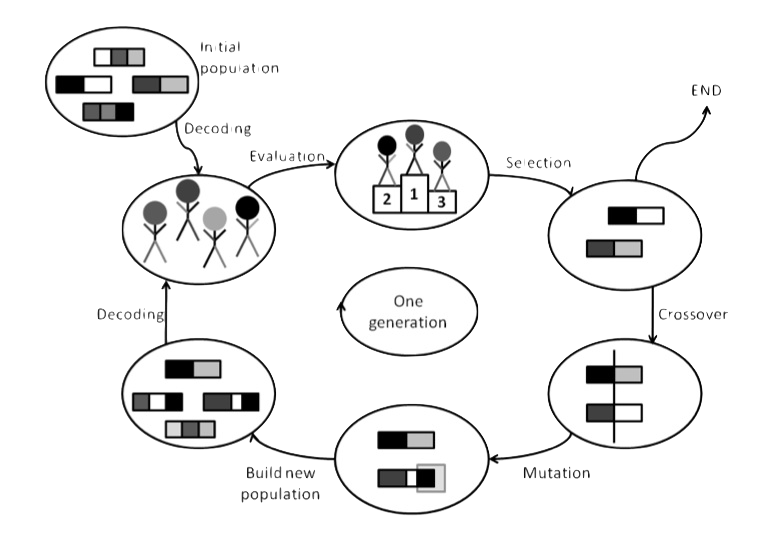
\includegraphics[width=0.8\textwidth]{img/working_principle_of_EA.png}
  \captionsetup{singlelinecheck=off,justification=raggedright}
  \caption{Schematic illustration of the evolutionary algorithm \cite[Figure 1]{Prothmann2009EvolutionaryOptimisation}}
\end{figure}
    
\end{frame}

\begin{frame}{Evolutionary Algorithms}
\begin{figure}
  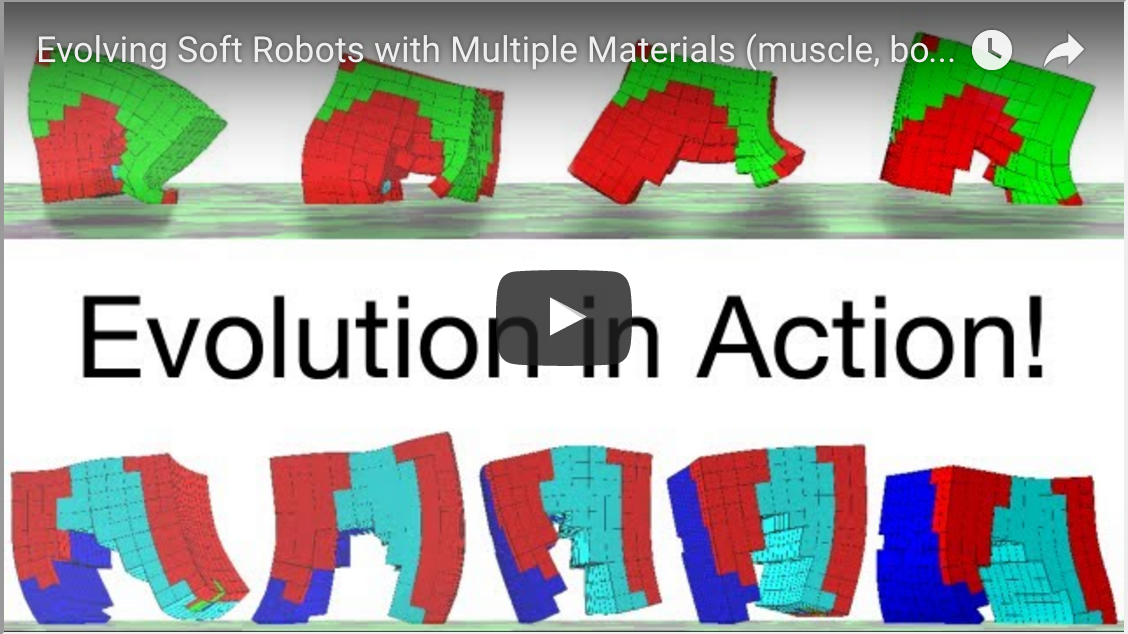
\includegraphics[width=0.8\textwidth]{img/evolution_in_action.png}
  \captionsetup{singlelinecheck=off,justification=raggedright}
\href{https://youtu.be/z9ptOeByLA4?t=1m08s}{\caption{Evolution in Action \cite{Cheney2013UnshacklingEncoding}}}
\end{figure}
\end{frame}

\begin{frame}{Evolutionary Algorithms: Glossary}
\begin{itemize}
  \item individual
  \item population
  \item fitness function
  \item selection
  \item recombination
  \item genotype
  \item phenotype
\end{itemize}
\end{frame}

\begin{frame}{Evolutionary Algorithms: Problem Statement}
  What makes an evolutionary algorithm work?
\end{frame}

\section{Defining Evolvability}

\begin{frame}{Defining Evolvability}
consensus: the amount of useful variation generated by the evolutionary process
\begin{itemize}
  \item evolvability as the ability to generate heritable variation
  \item evolvability as bias towards useful variation
\end{itemize}
\end{frame}


\subsection{Evolvability as Heritable Variation}

\begin{frame}{Evolvability as Heritable Variation}
	\begin{figure}
 \centering
    \begin{subfigure}[b]{0.5\textwidth}
        \centering
    	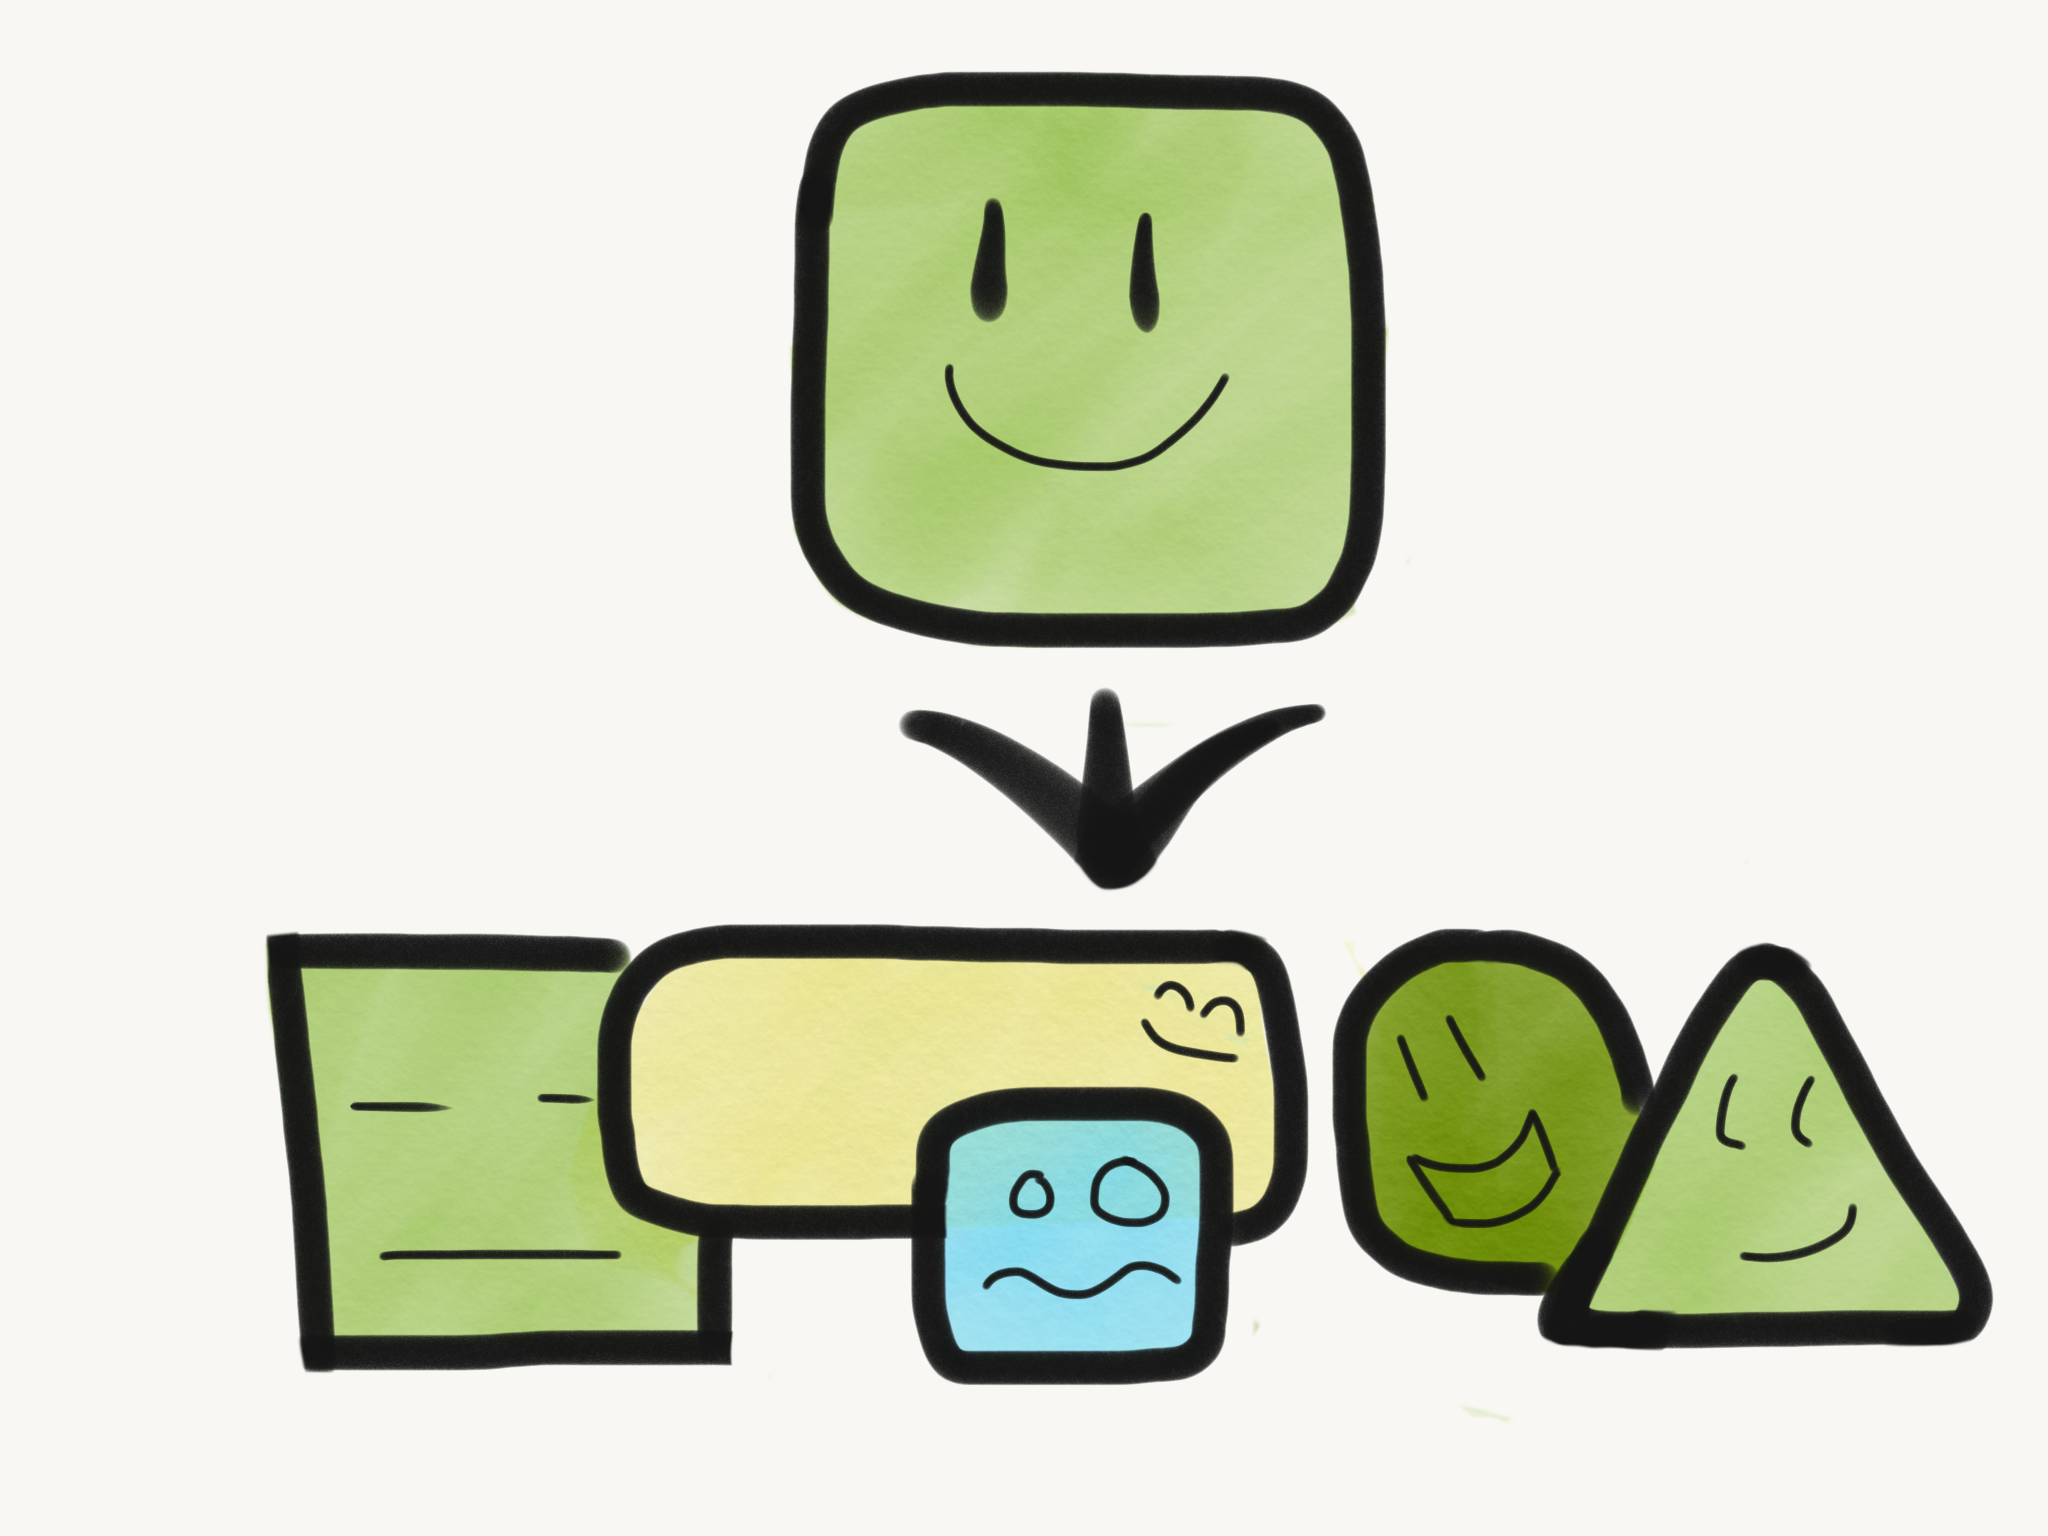
\includegraphics[width=\textwidth]{img/individual_evolvability.png}
        \caption{high individual evolvability}
        \label{subfig:canalization}
    \end{subfigure}%
    \hfill
    \begin{subfigure}[b]{0.5\textwidth}
        \centering
        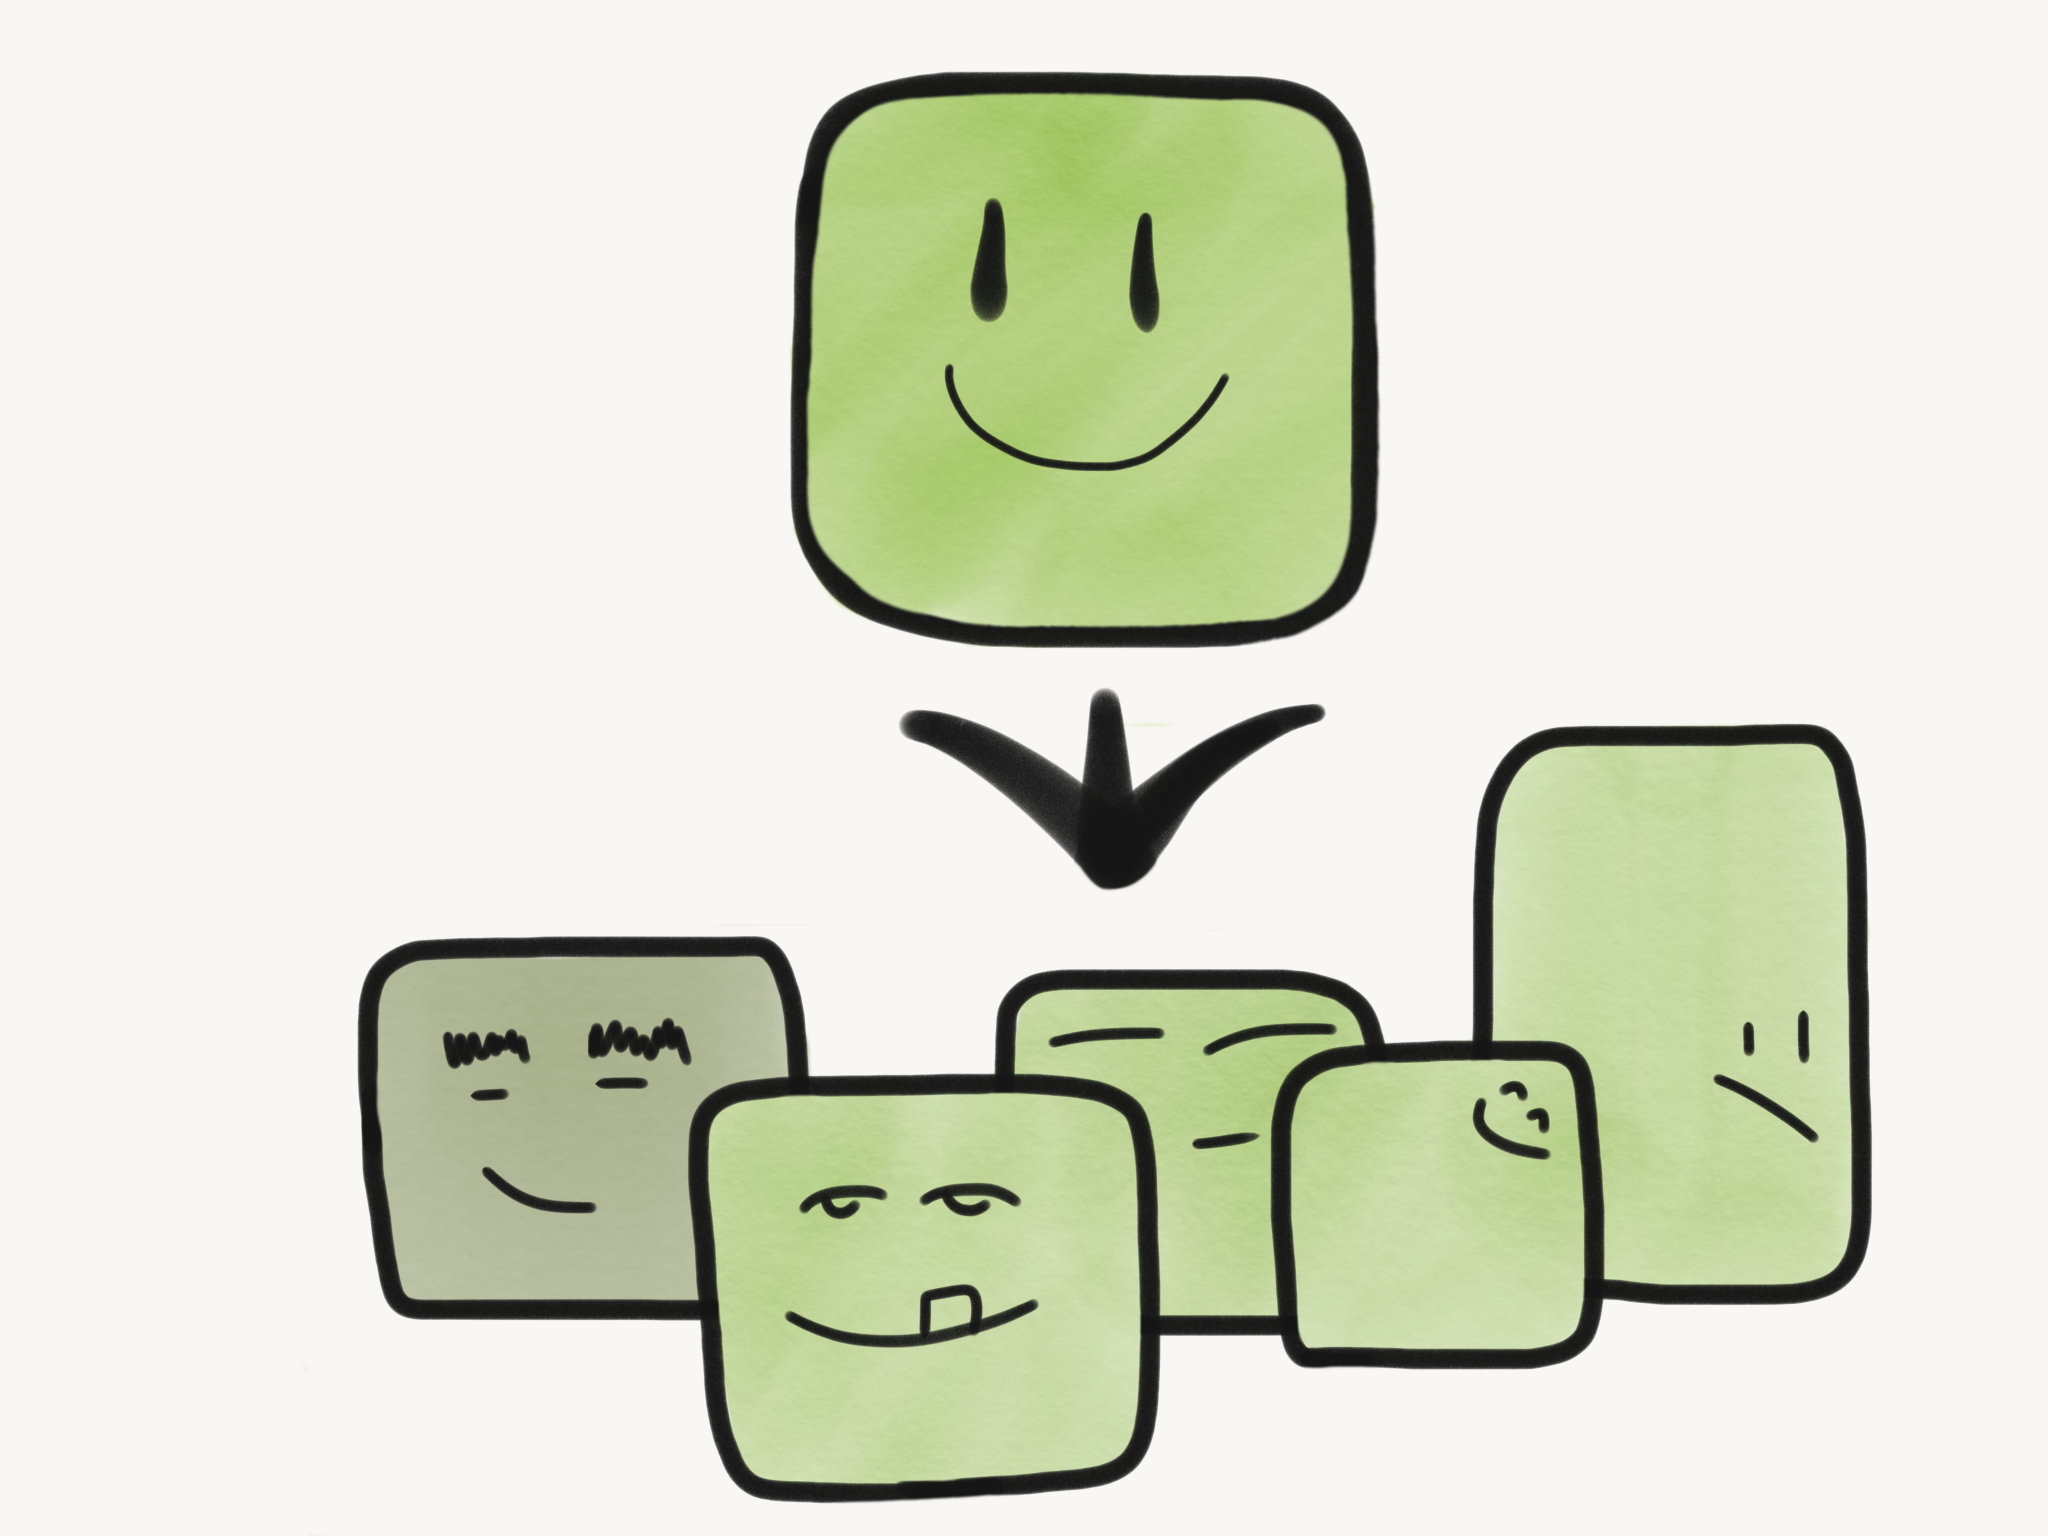
\includegraphics[width=\textwidth]{img/low_individual_evolvability.png}
        \caption{low individual evolvability}
        \label{subfig:no_canalization}
    \end{subfigure}
 	\captionsetup{singlelinecheck=off,justification=raggedright}
    \vspace{-4ex}
  \captionsetup{singlelinecheck=off,justification=raggedright}
  \caption{An illustration of individual evolvability, considering evolvability as heritable variation \cite{Wilder2015ReconcilingEvolvability}.}
  \label{fig:high_vs_low_individual_evolvability}
\end{figure}
\end{frame}

\subsection{Evolvability as Bias towards Useful Variation}

\begin{frame}{Evolvability as Bias towards Useful Variation}
  \begin{figure}
    \centering
    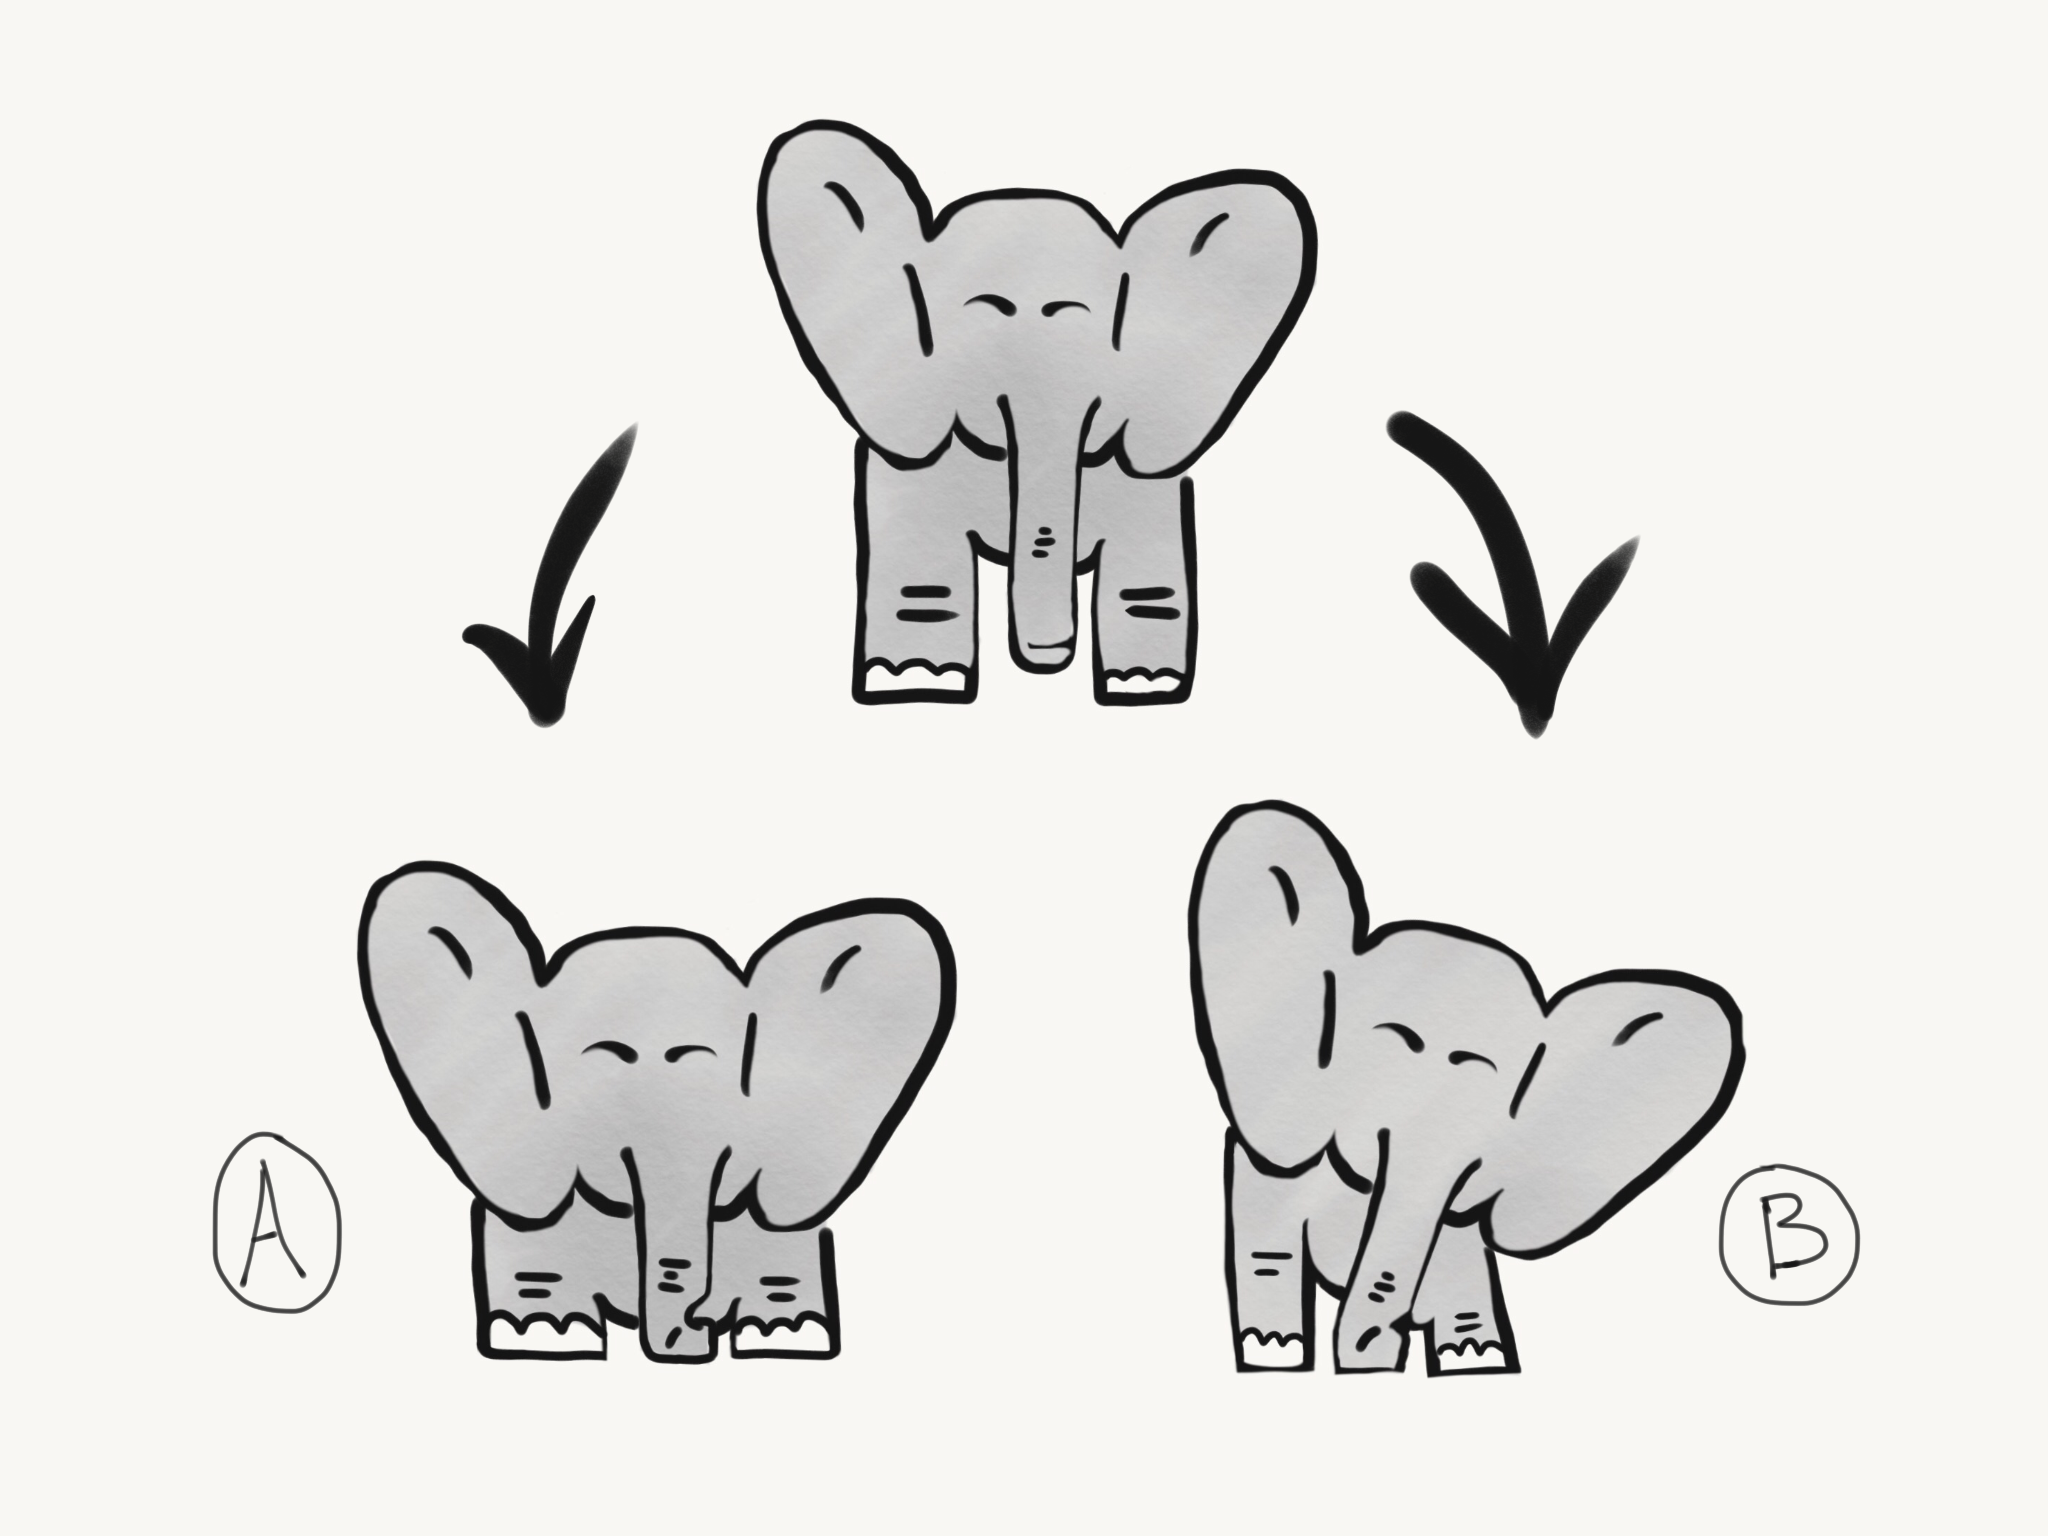
\includegraphics[width=0.8\textwidth]{img/developmental_constraint}
 	\captionsetup{singlelinecheck=off,justification=raggedright}
  	\caption{Illustration of developmental constraint; high evolvability left and low evolvability right \cite{Smith1985DevelopmentalBiology,Tuinstra1990LackDevelopment}.}
    \label{fig:developmental_constraint}
\end{figure}
\end{frame}

\begin{frame}{Evolvability as Bias towards Useful Variation}
  \begin{figure}
    \centering
    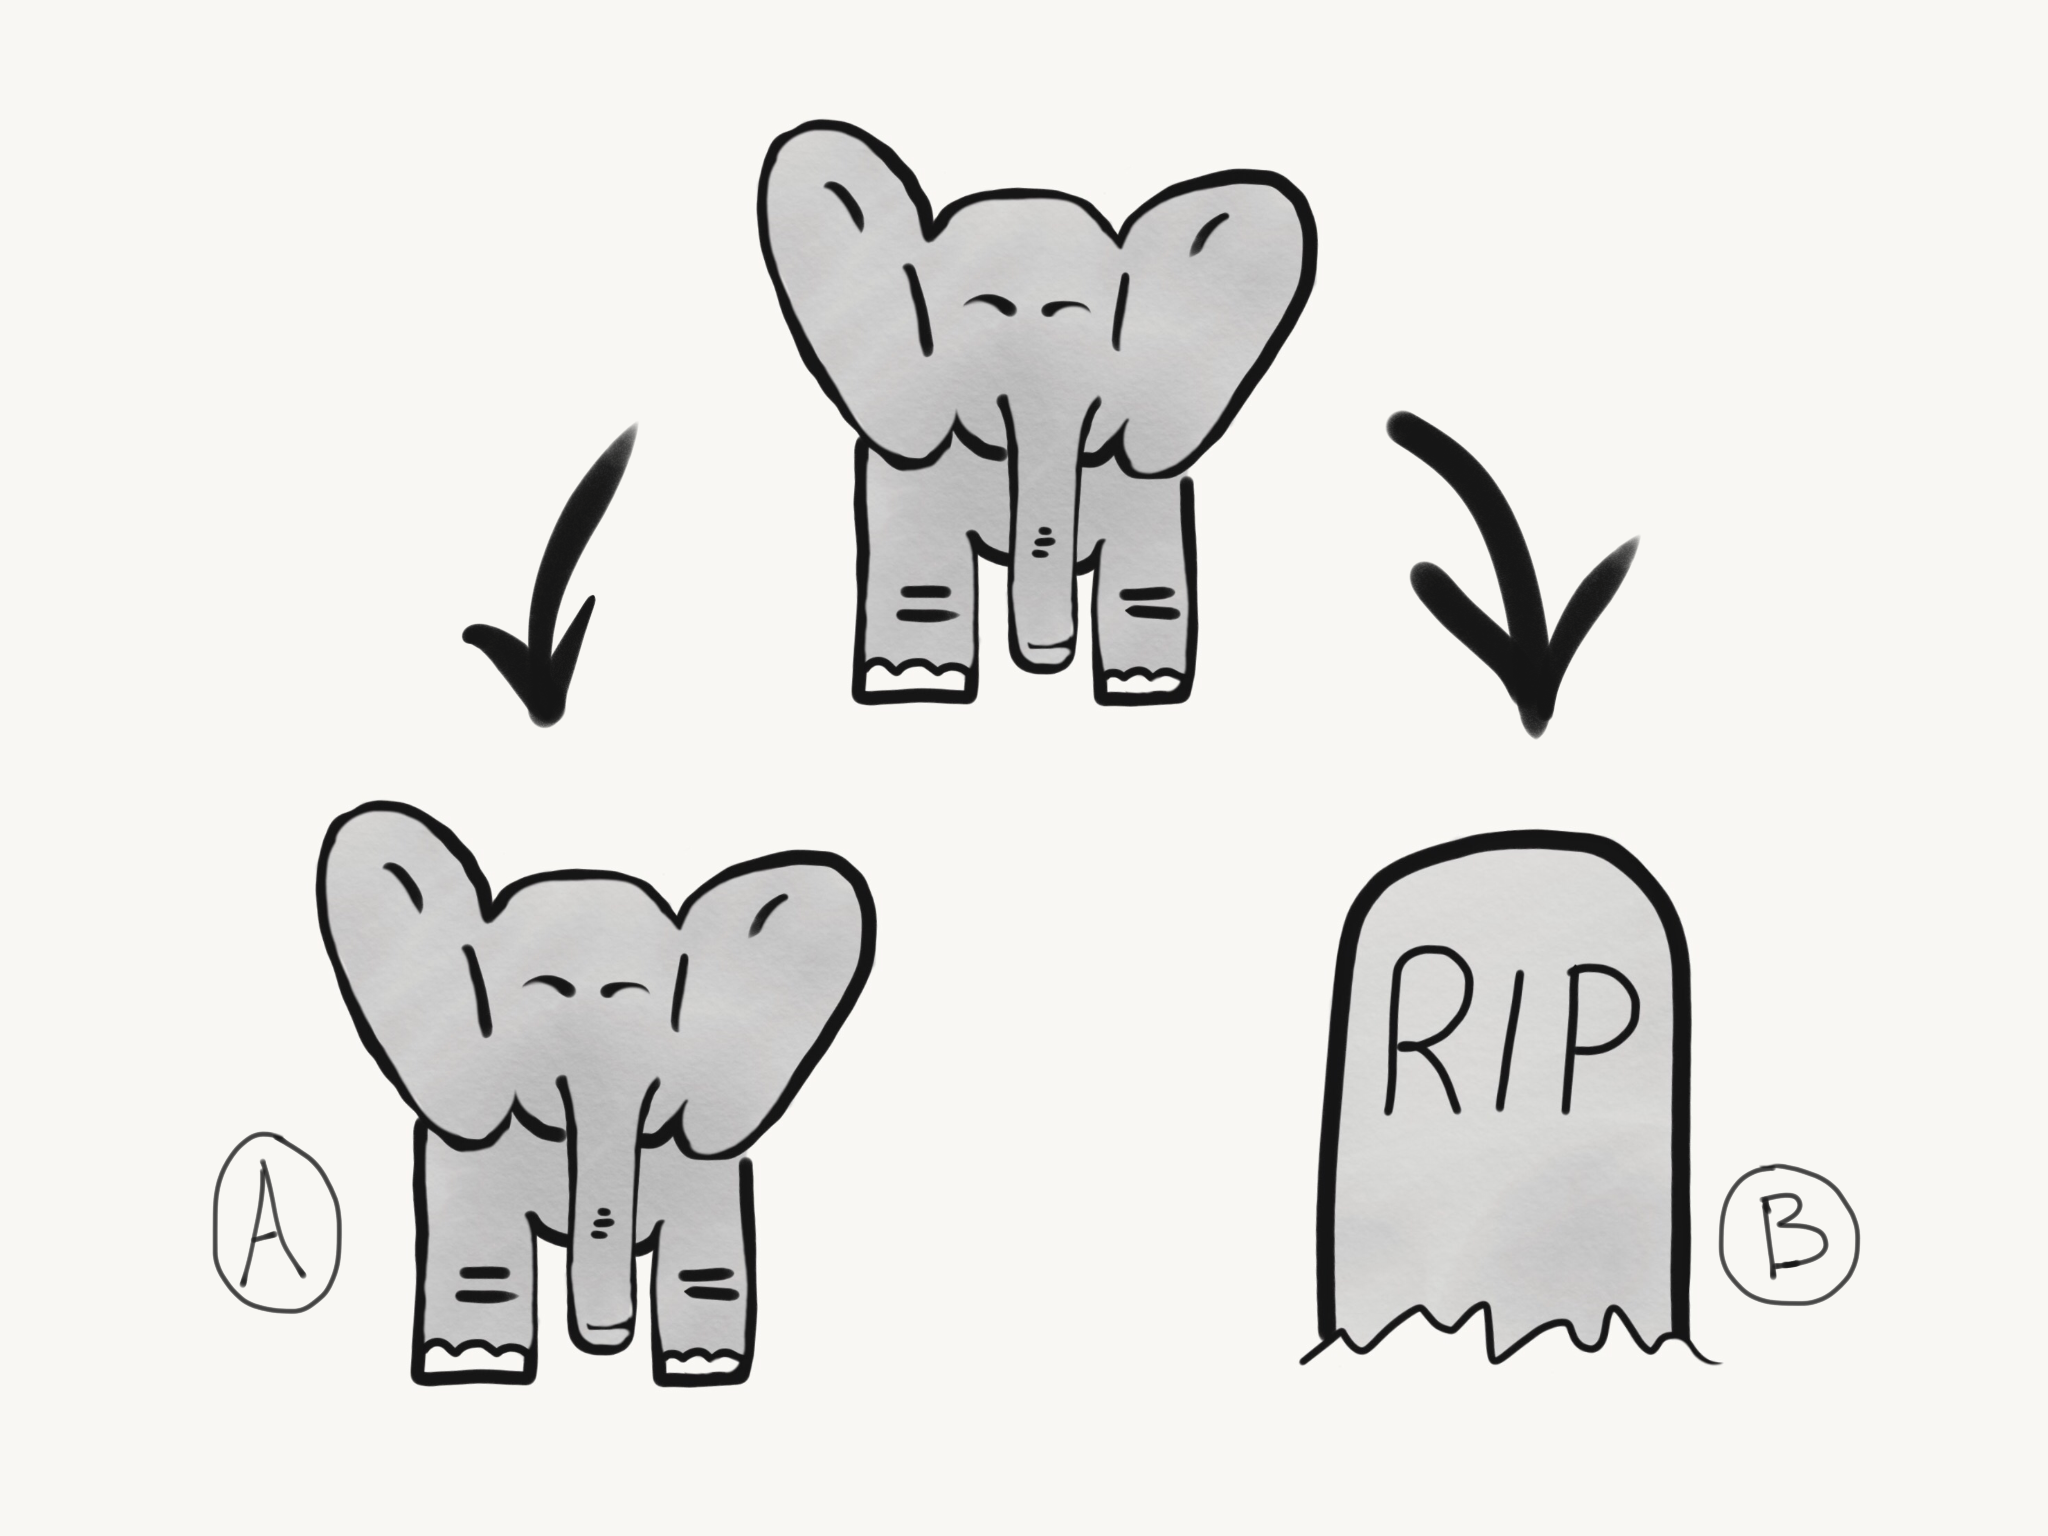
\includegraphics[width=0.8\textwidth]{img/robustness}
 	\captionsetup{singlelinecheck=off,justification=raggedright}
  	\caption{Illustration of robustness; high evolvability left and low evolvability right \cite{Downing2015IntelligenceSystems}.}
    \label{fig:robustness}
\end{figure}
\end{frame}


\section{Experiment Design}

\begin{frame}{Development and the Environment}
\begin{columns}
\column{0.5\textwidth}
neglecting environmental influence
\begin{align*}
\vec{p} = f(\vec{g})
\end{align*}
\column{0.5\textwidth}
considering environmental influence
\begin{align*}
\vec{p} = f(\vec{g}, \vec{e})
\end{align*}
\end{columns}
\end{frame}

\begin{frame}{Development and the Environment: Direct Plasticity}
  \begin{figure} \label{fig:elephant_developmental_perturbation}
  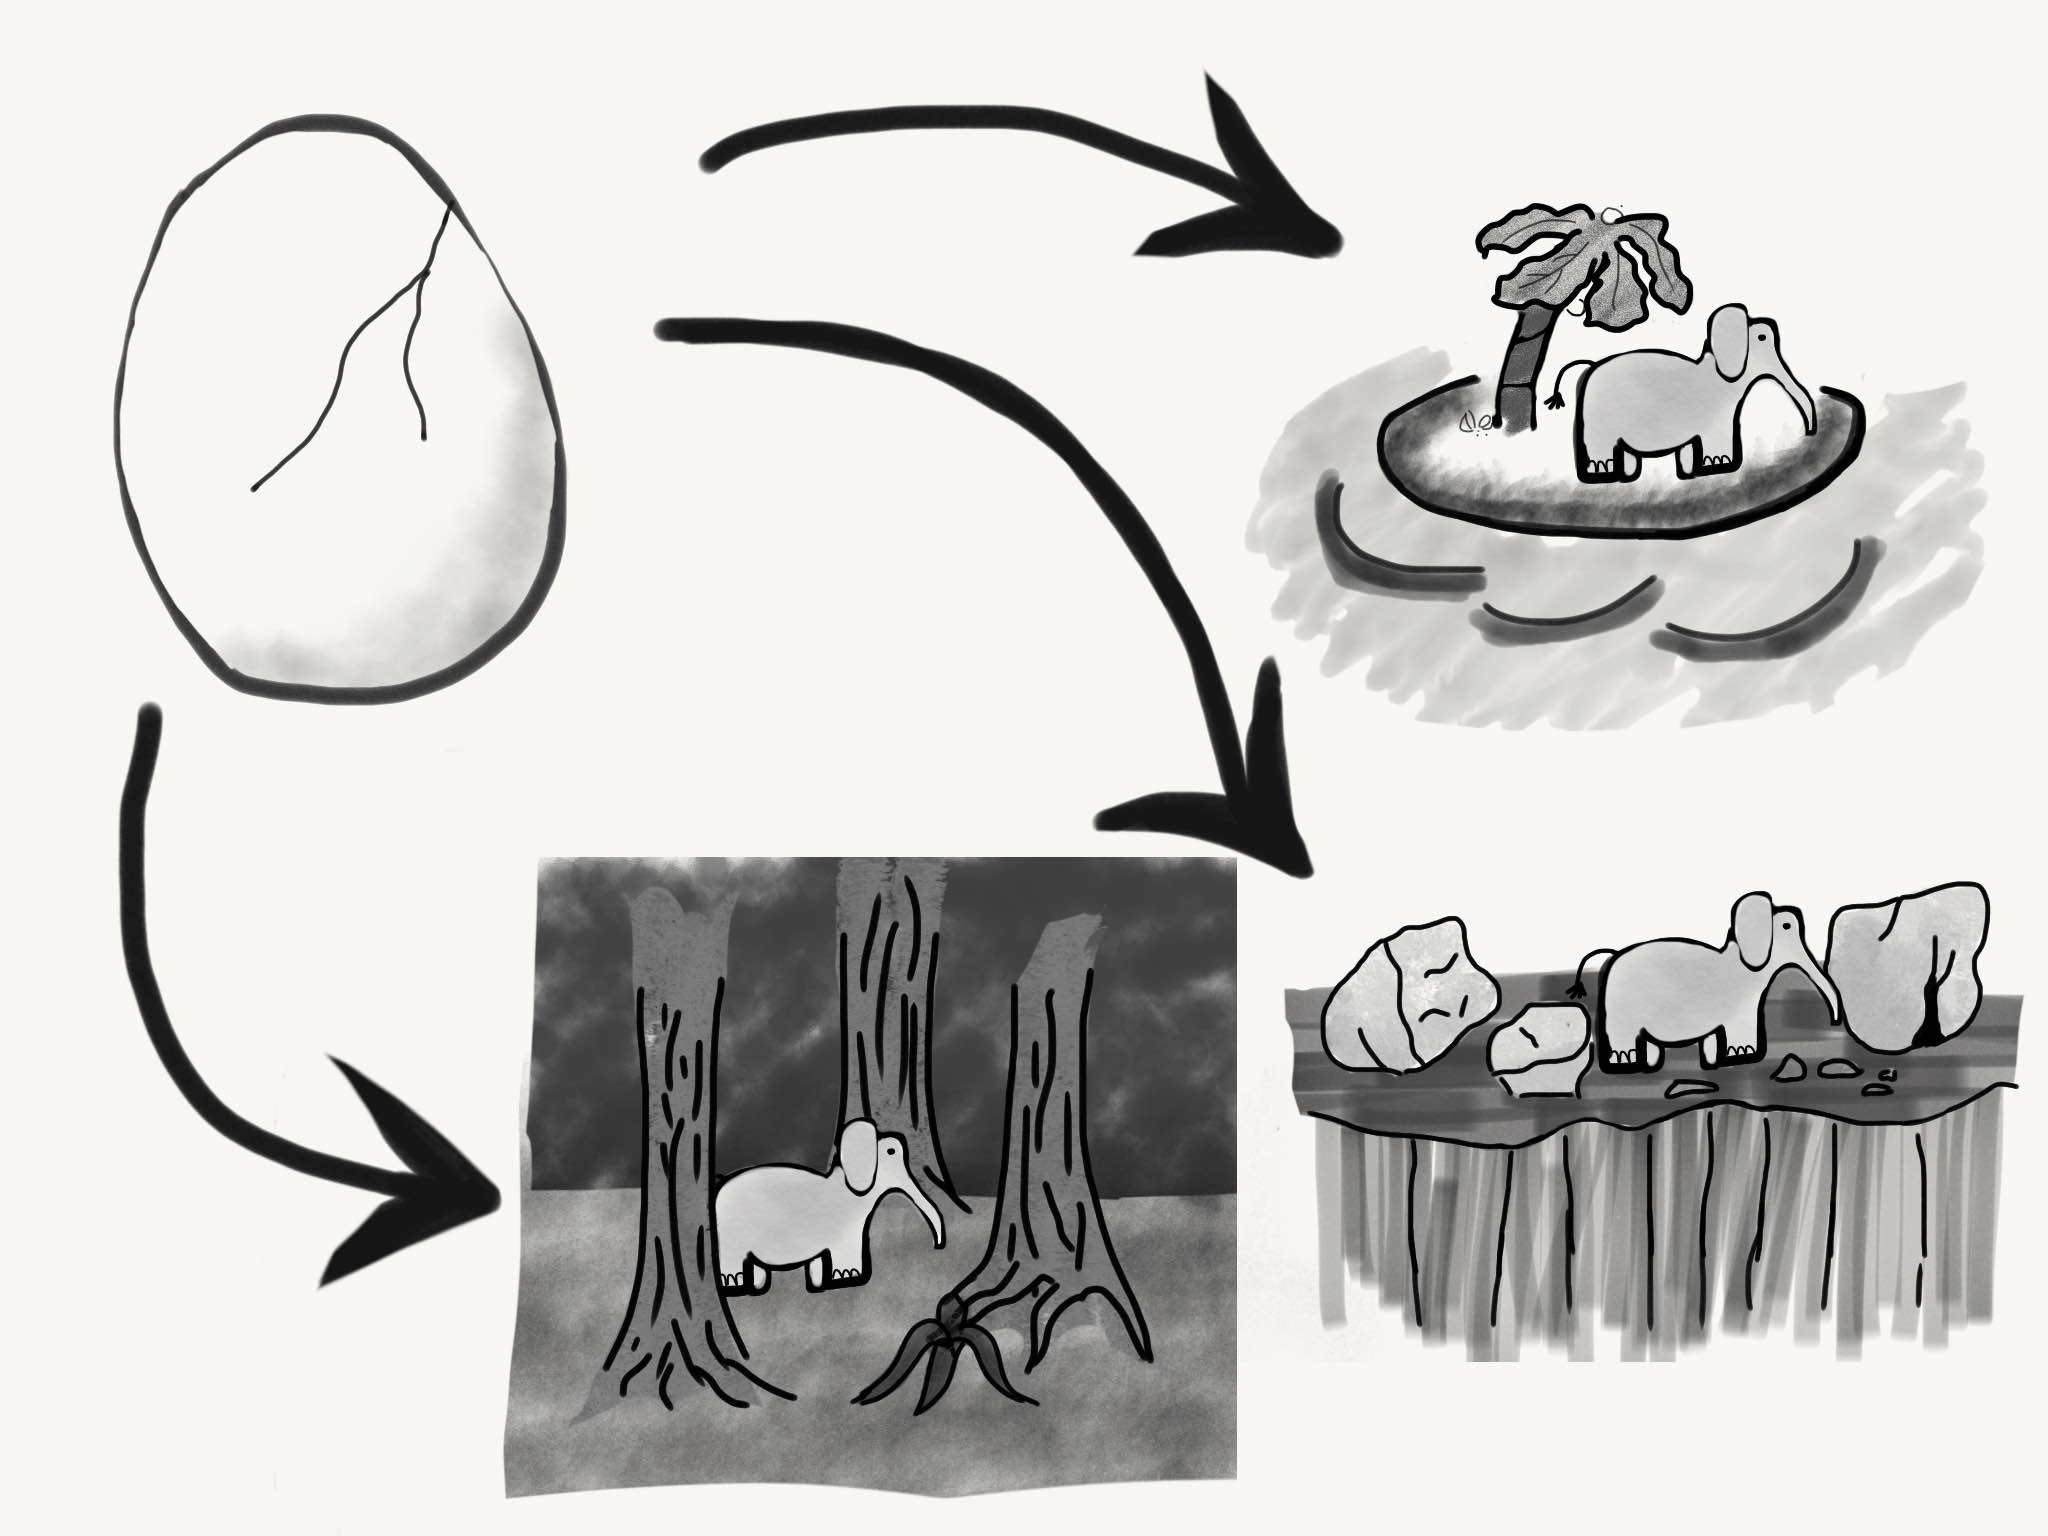
\includegraphics[width=0.8\textwidth]{img/elephant_developmental_perturbation.jpg}
  \captionsetup{singlelinecheck=off,justification=raggedright}

  \caption{An illustration of canalization against environmental perturbation}
\end{figure}
\end{frame}

\begin{frame}{Development and the Environment: Direct Plasticity}
goal is $\dot{\vec{g}}$ such that
\begin{align*}
\vec{p} \approx f(\dot{\vec{g}}, \vec{e})  \approx f(\dot{\vec{g}}, \vec{e} + \bm{\vec{n}})
\end{align*}
\end{frame}

\begin{frame}{Development and the Environment: Indirect Plasticity}
  \begin{figure} \label{figs/plant_developmental_perturbation}
  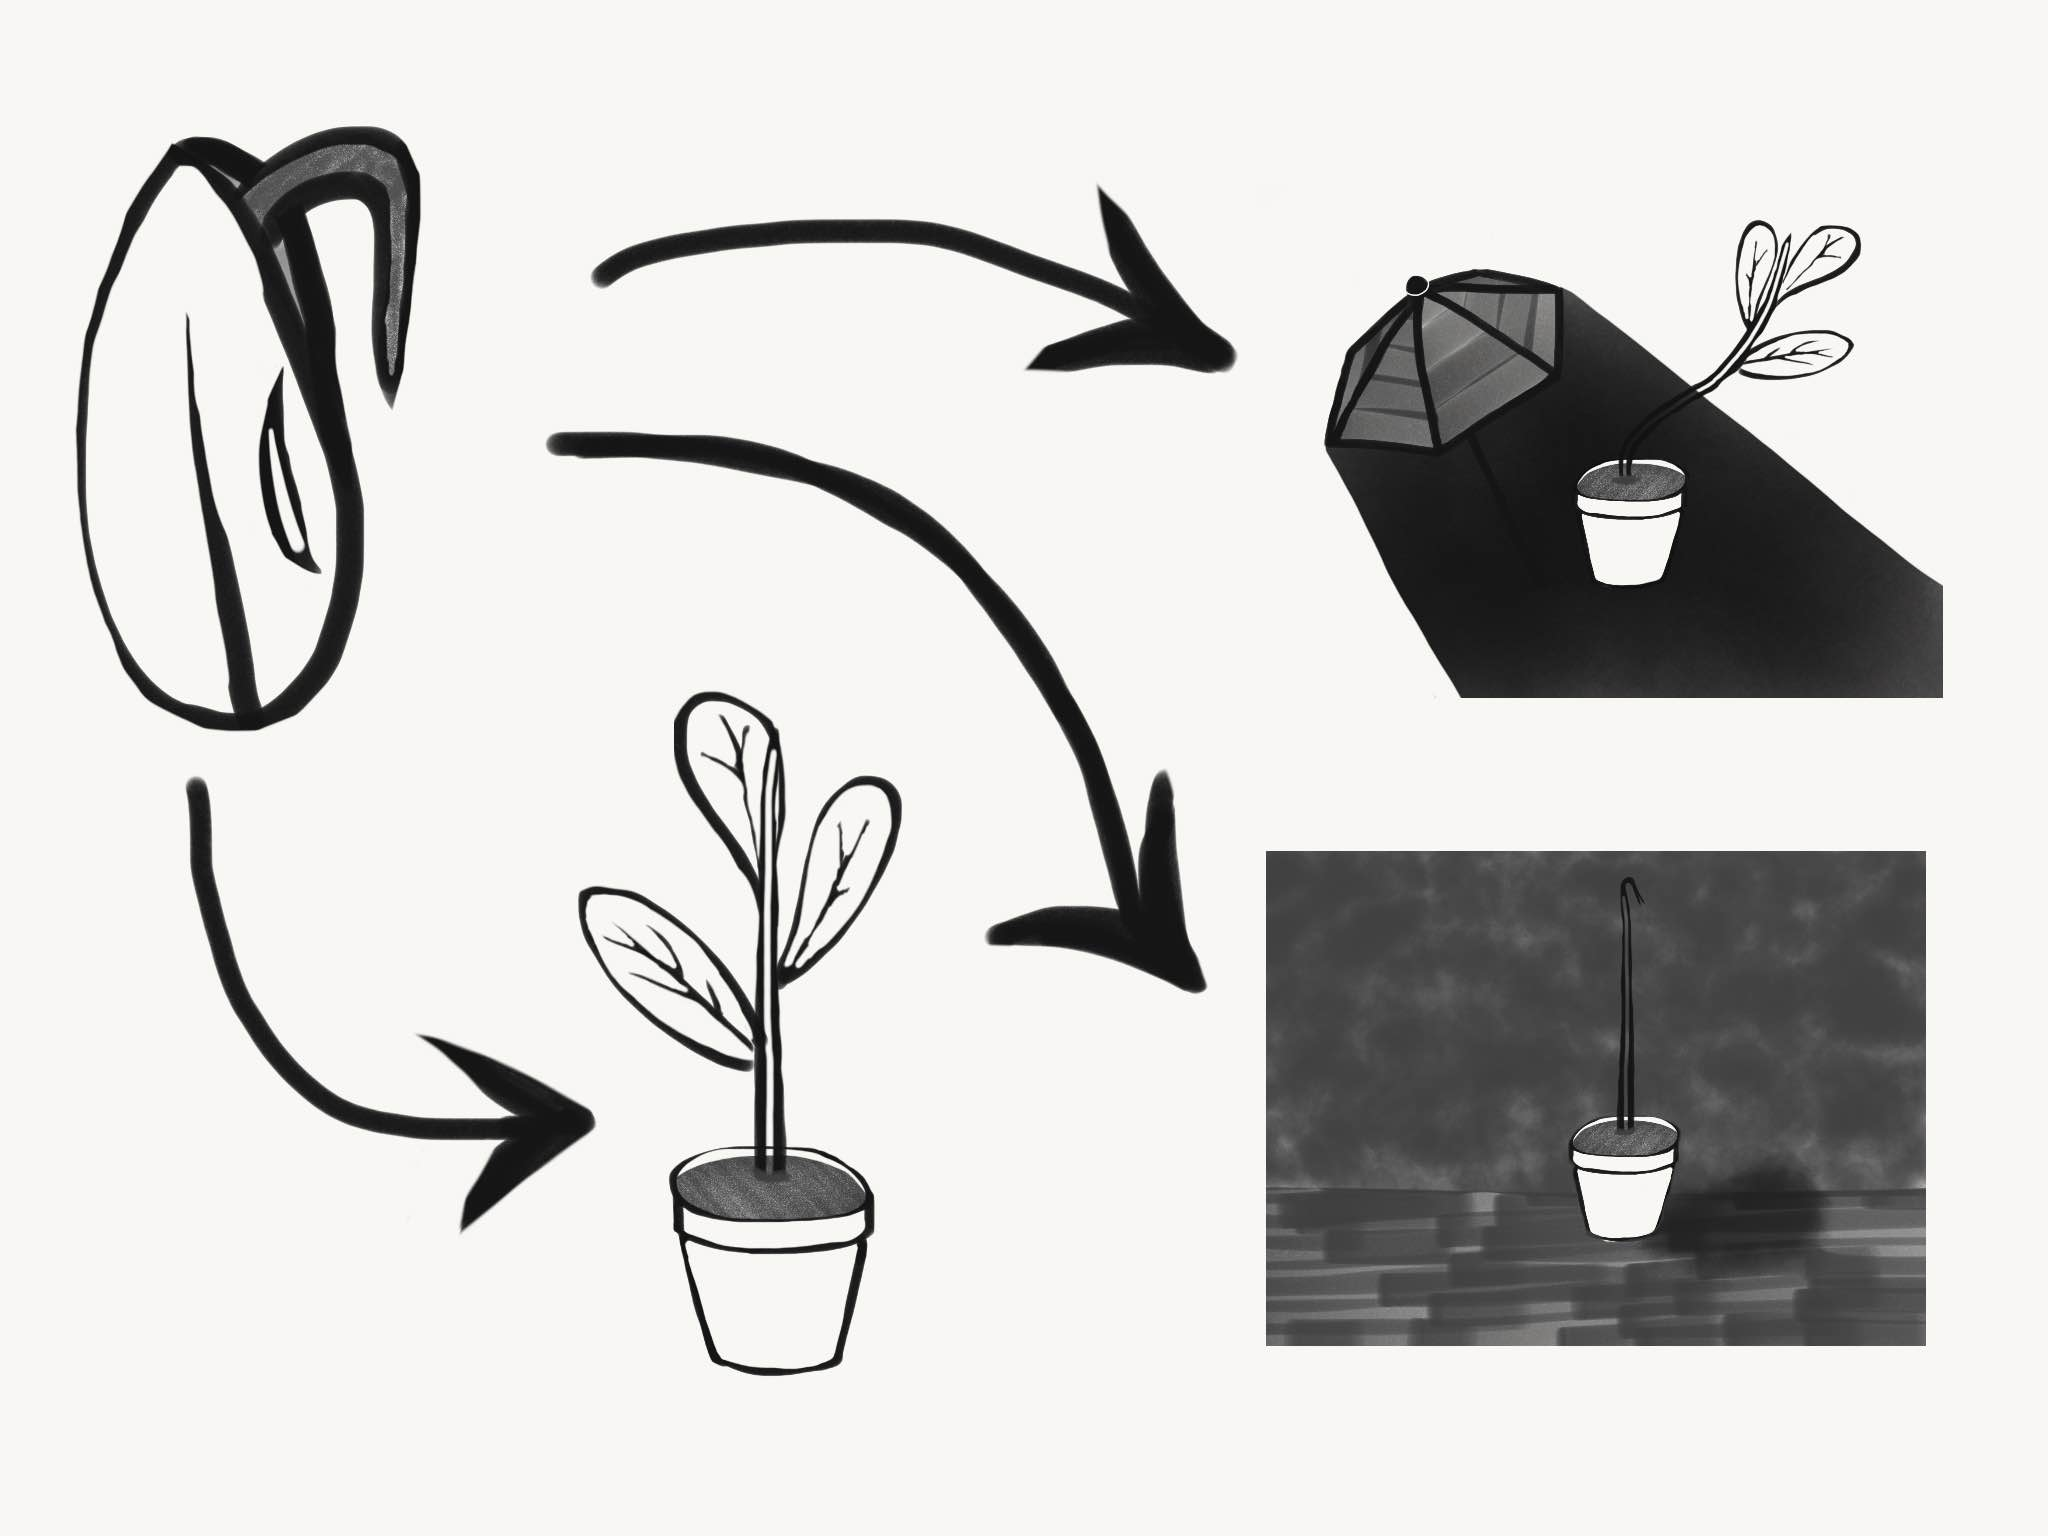
\includegraphics[width=0.8\textwidth]{img/plant_developmental_perturbation.jpg}
  \captionsetup{singlelinecheck=off,justification=raggedright}
  \caption{An illustration alternate phenotypes expressed based on environmental signals}
\end{figure}

\end{frame}

\begin{frame}{Development and the Environment: Indirect Plasticity}
goal is $\dot{\vec{g}}$ such that:
\begin{align*}
\vec{p}_1 &\approx f(\hat{\vec{g}}, \vec{e} + \vec{e}_1) \\
\vec{p}_2 &\approx f(\hat{\vec{g}}, \vec{e} + \vec{e}_2) \\
&\vdotswithin{\approx} \\
\vec{p}_s &\approx f(\hat{\vec{g}}, \vec{e} + \vec{e}_s)
\end{align*}
\end{frame}

\begin{frame}{GRN Models}
  \begin{itemize}
    \item Model A \cite{Wilder2015ReconcilingEvolvability}
	 \begin{align*}
    	W_{i,j} \in \{-1,0,1\} \\
        S_i \in \{0,1\}
    \end{align*}
    \begin{align*}
    S_i(t+1) = 
      \begin{cases}
      1 & \text{if } \sum_{j=1}^{k} W_{ji}S_j(t) > 0 \\
      0 & \text{otherwise.}
      \end{cases}
    \end{align*}
    \item Model B \cite{Kuo2006NetworkDivergence}
  \end{itemize}
\end{frame}

\section{Experiment Progress}

\begin{frame}{Experiment Progress}
\begin{itemize}
  \item \textbf{Week 1} (January 16th) -- Work on proposal \checkmark, play with DEAP \checkmark
  \item \textbf{Week 2} (January 23rd) -- Code and test first model \checkmark
  \item \textbf{Week 3} (January 30th) -- Code and test second model (part I) \ding{55}, Run first model \checkmark
  \item \textbf{Week 4} (February 6th) -- Code and test second model (part II) \ding{55}, Analyze data from first model \checkmark, Plan adjustments to experimental protocol \checkmark
  \item \textbf{Week 5} (February 13th) -- Code and test second model (part III) \ding{55}
  \item \textbf{Week 6} (February 20th) -- Run second model
  \item \textbf{Week 7} (February 27th) -- Analyze data from second model
  \item \textbf{Week 8} (March 6th) -- Further experimental tweaks and data collection
  \item \textbf{Week 9} (March 13th) -- Spring Break, Prepare for thesis presentation, Complete data collection
\end{itemize}
\vspace{-1ex}
\begin{center}
{\centering ~$\bm{\vdots}$~}
\end{center}
\end{frame}

\appendix


\begin{frame}[standout]
  Questions?
\end{frame}

\begin{frame}[allowframebreaks]{References}

  \bibliography{Mendeley}
  \setbeamertemplate{bibliography item}{\insertbiblabel}
  %\nocite{*} % Insert publications even if they are not cited in the poster
  \bibliographystyle{apalike}
\end{frame}

\begin{frame}{Bio AI}
\begin{figure}
  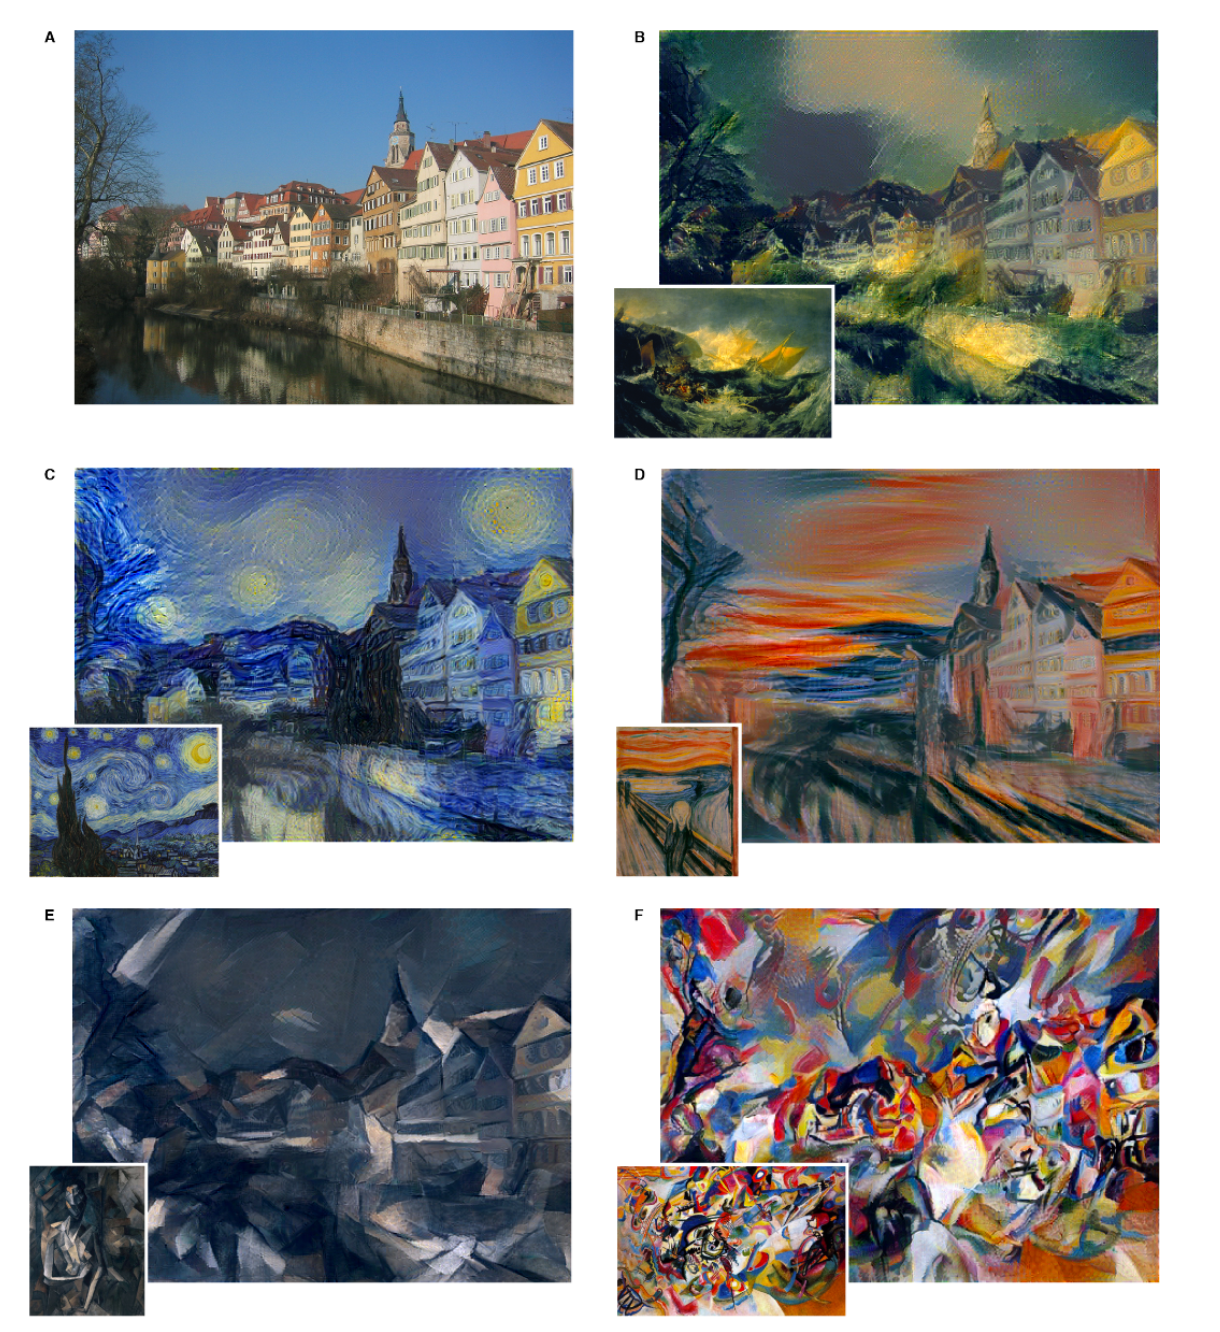
\includegraphics[width=0.6\textwidth]{img/nn_art_styles.png}
  \captionsetup{singlelinecheck=off,justification=raggedright}
  \caption{A Neural Algorithm of Artistic Style \cite{Gatys2015AStyle}}
\end{figure}
\end{frame}

\begin{frame}{Evolvability as Heritable Variation}
  \begin{figure}
 \centering
    \begin{subfigure}[b]{0.5\textwidth}
        \centering
    	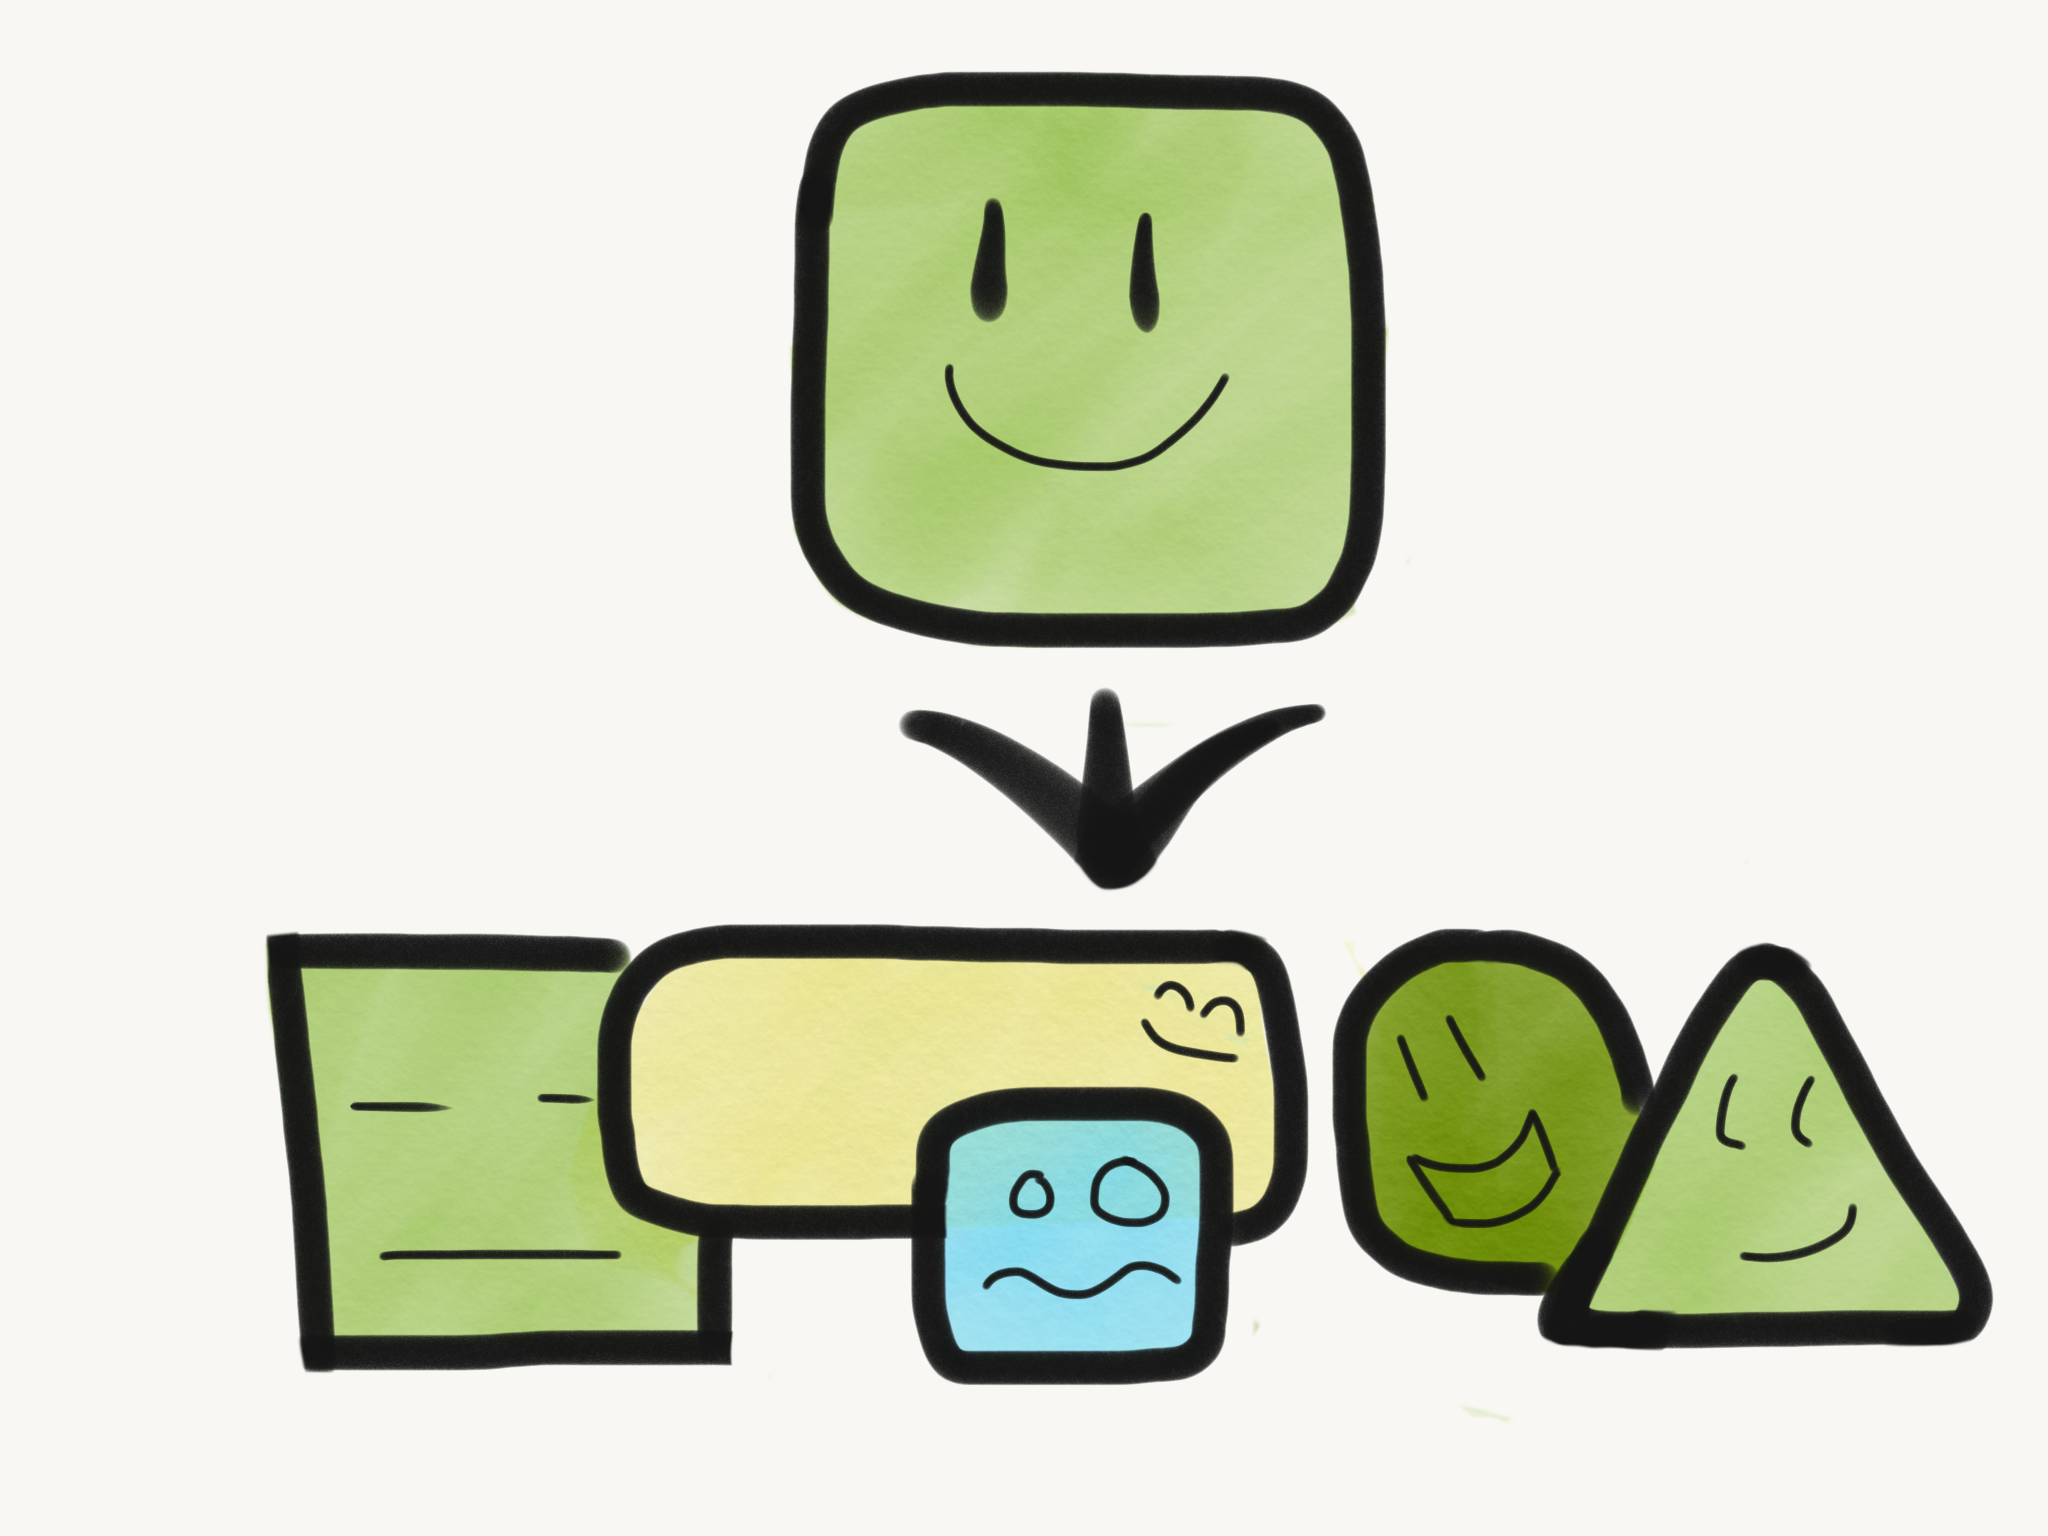
\includegraphics[width=\textwidth]{img/individual_evolvability}
        \caption{individual evolvability}
        \label{subfig:individual_evolvability}
    \end{subfigure}%
    \hfill
    \begin{subfigure}[b]{0.5\textwidth}
        \centering
        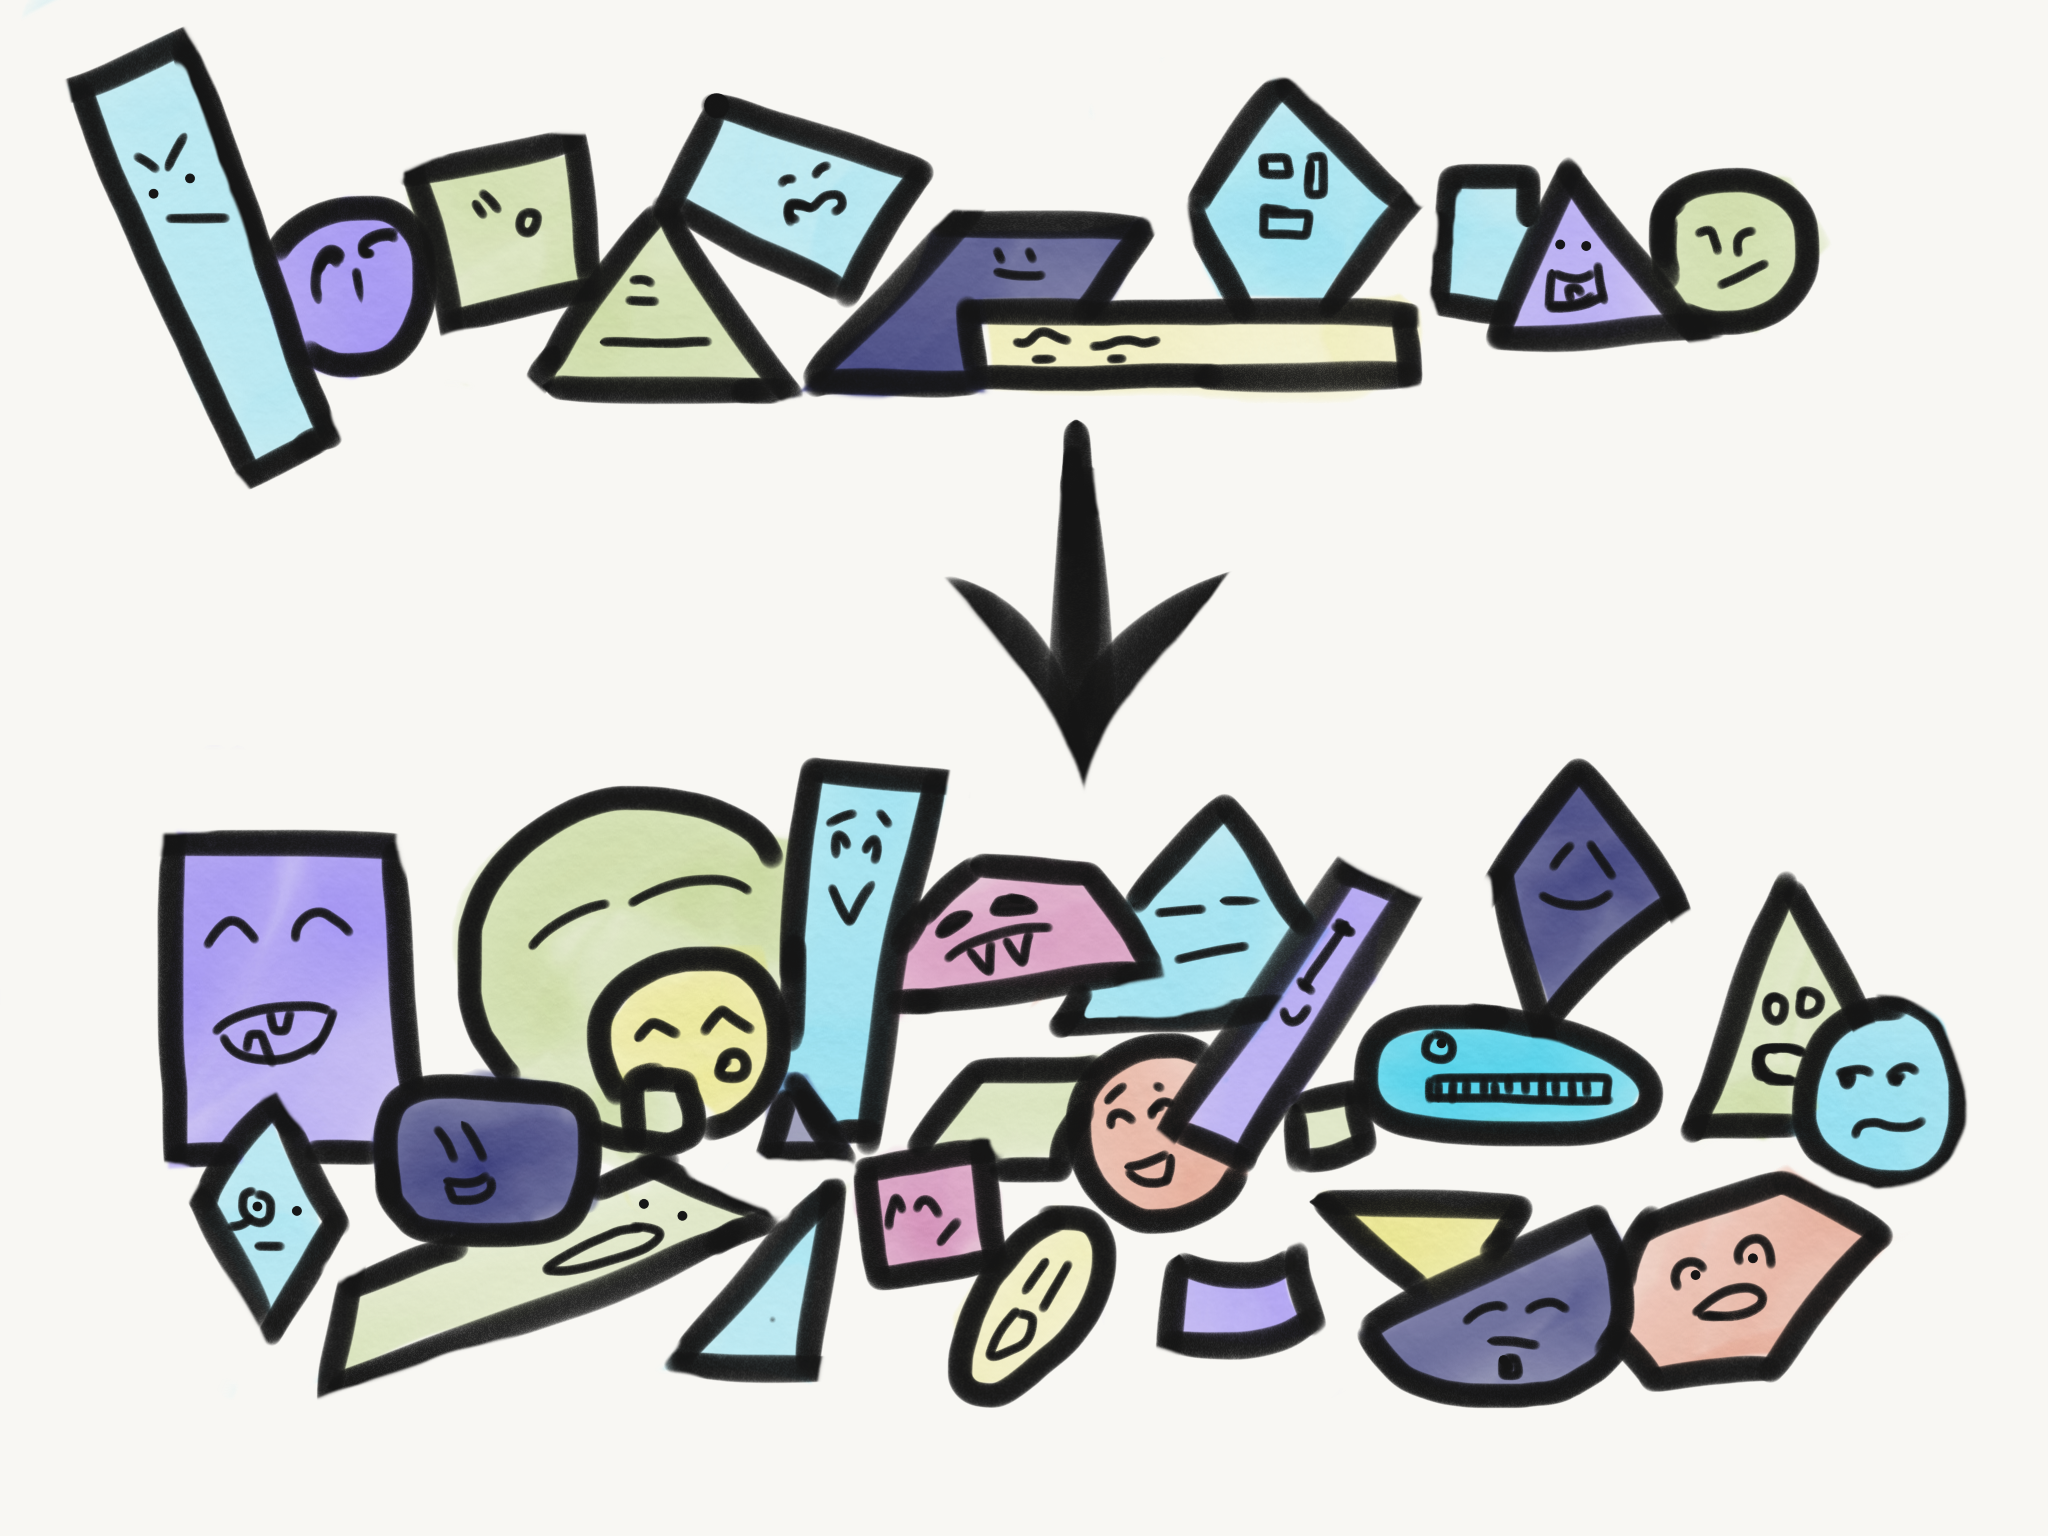
\includegraphics[width=\textwidth]{img/population_evolvability}
        \caption{population evolvability}
        \label{subfig:population_evolvability}
    \end{subfigure}
 	\captionsetup{singlelinecheck=off,justification=raggedright}
    \vspace{-4ex}
  \captionsetup{singlelinecheck=off,justification=raggedright}
  \caption{An illustration contrasting individual and population evolvability \cite{Wilder2015ReconcilingEvolvability}.}
  \label{fig:individual_vs_population_evolvability}
\end{figure}
\end{frame}

\begin{frame}{Evolvability as Bias towards Useful Variation}
  \begin{figure}
    \centering
    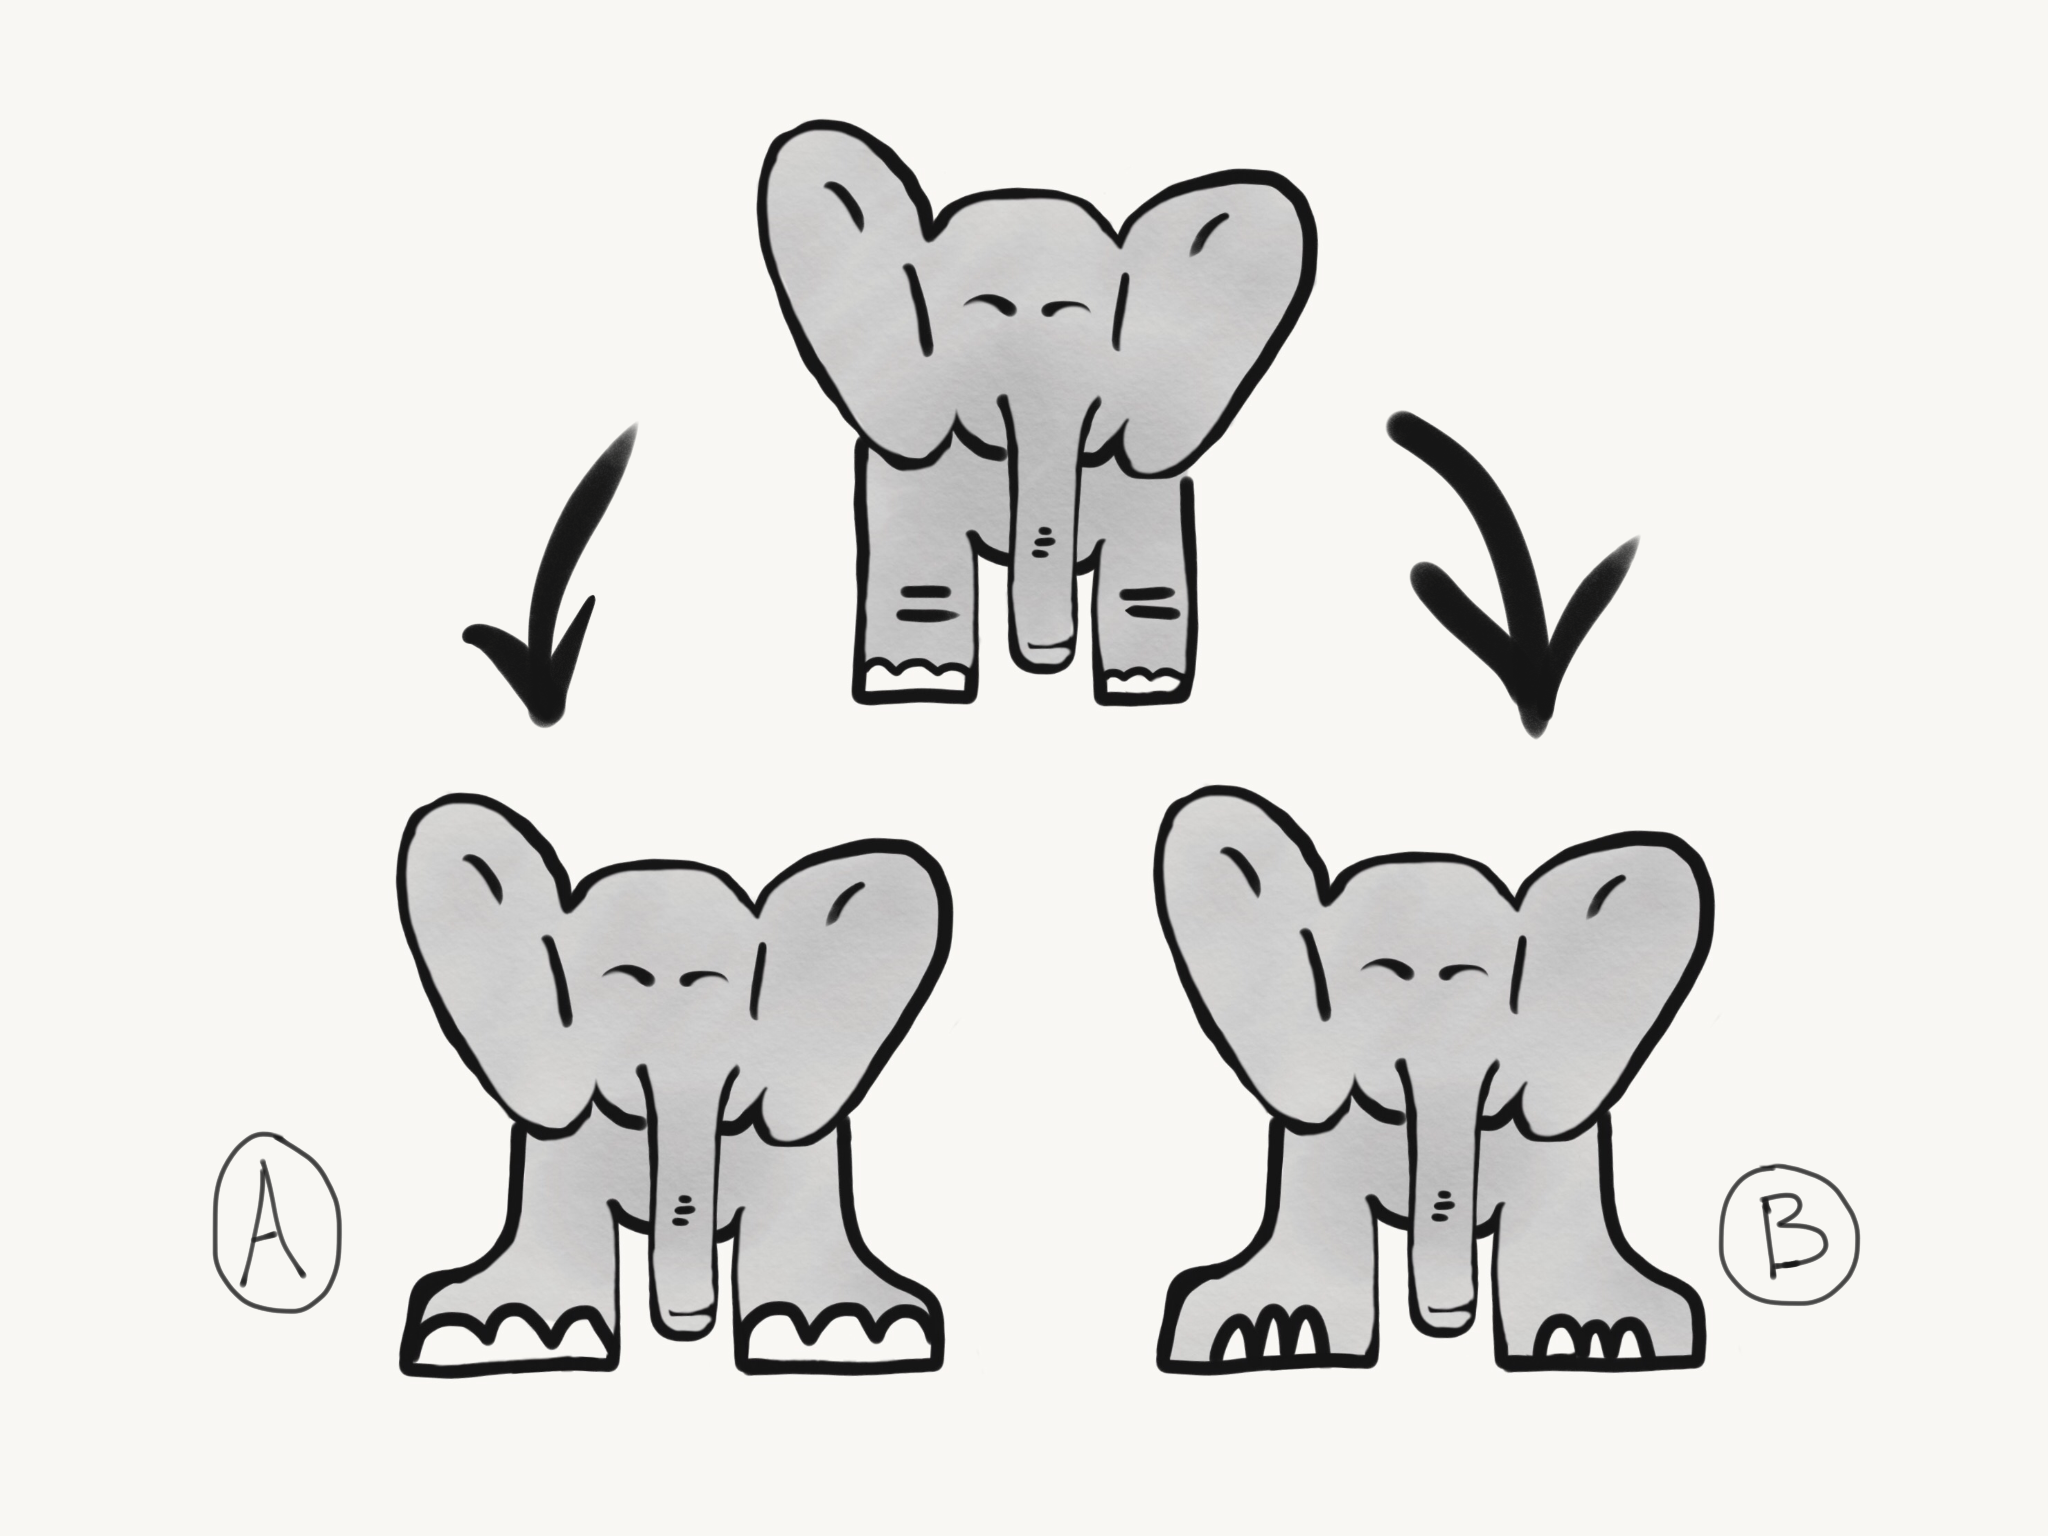
\includegraphics[width=0.8\textwidth]{img/exploratory_growth}
 	\captionsetup{singlelinecheck=off,justification=raggedright}
  	\caption{Illustration of exploratory growth; high evolvability left and low evolvability right \cite{Downing2015IntelligenceSystems}.}
    \label{fig:exploratory_growth}
\end{figure}
\end{frame}

\begin{frame}{Evolvability as Bias towards Useful Variation}
  \begin{figure}
    \centering
    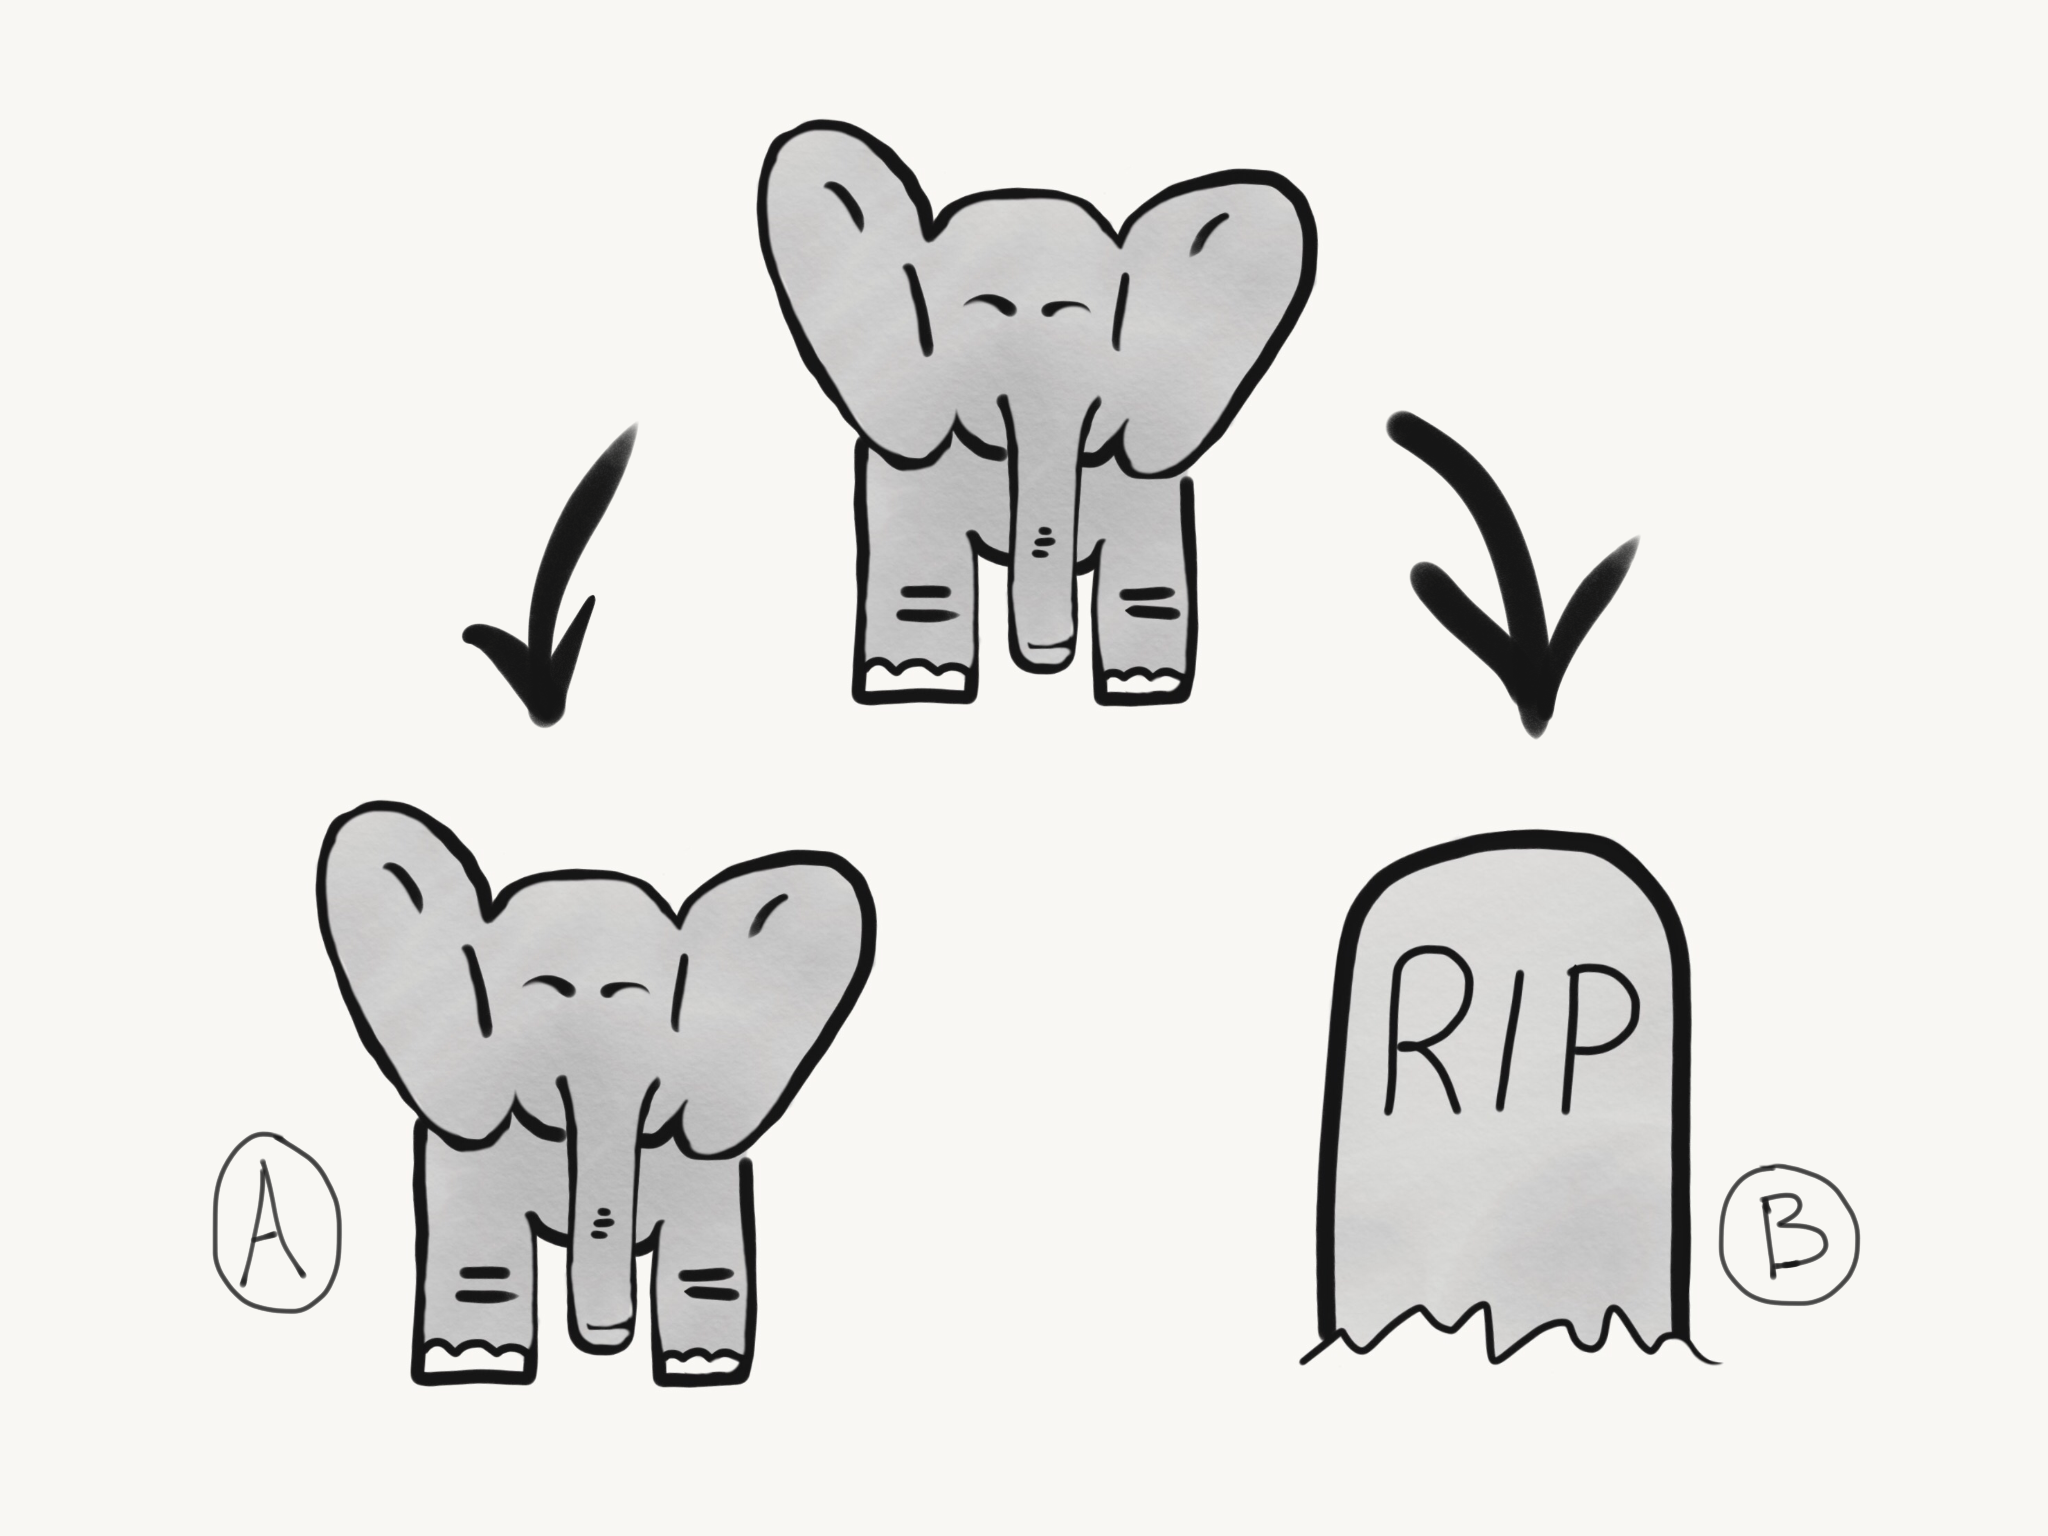
\includegraphics[width=0.8\textwidth]{img/robustness}
 	\captionsetup{singlelinecheck=off,justification=raggedright}
  	\caption{Illustration of robustness; high evolvability left and low evolvability right \cite{Downing2015IntelligenceSystems}.}
    \label{fig:robustness}
\end{figure}
\end{frame}

\begin{frame}{Selection Pressure}
\begin{figure}
\resizebox{\textwidth}{!}{%
	\pgfmathsetseed{1}
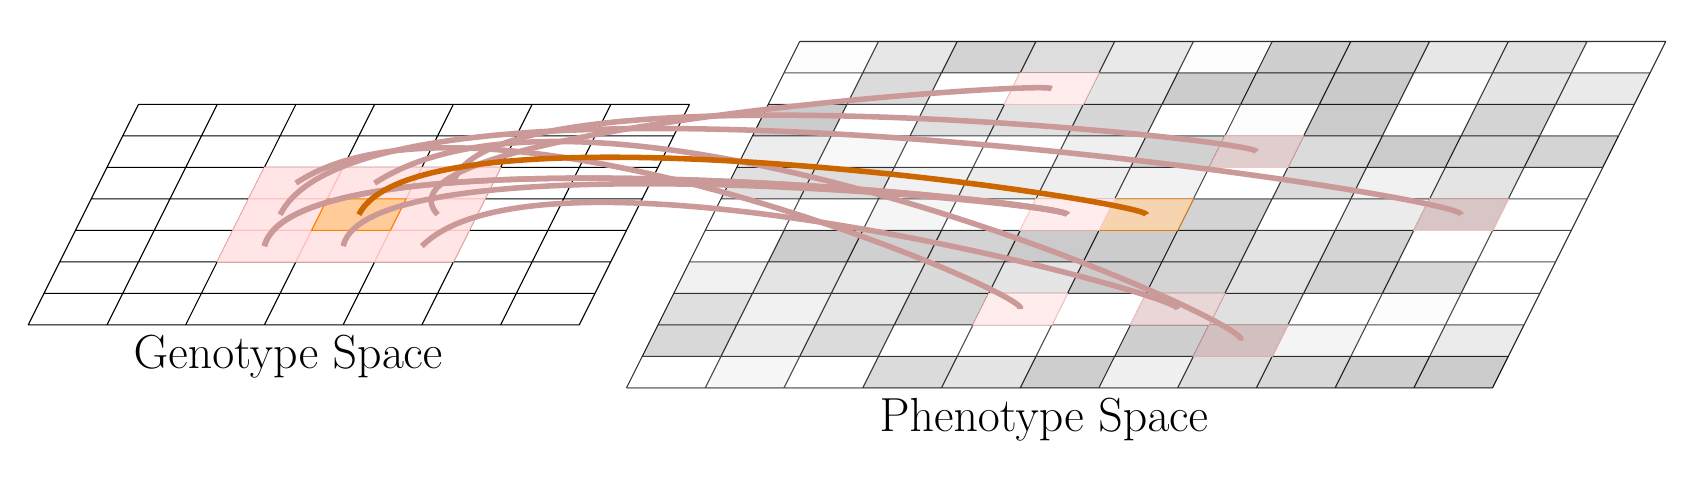
\begin{tikzpicture} [x={(-0.2cm,-0.4cm)}, y={(1cm,0cm)}, z={(0cm,1cm)}, scale=1]   

   \begin{scope}[canvas is yx plane at z=0]
     \draw [black!100] (0,2) grid (7,9);
     \draw [black!100] (8,0) grid (19,11);
     
     % primary phenotype mapping
     \foreach \x in {2,3,4}
       \foreach \y in {4,5,6}
    	  \filldraw[fill=pink!40!white, draw=pink] (\x, \y) rectangle (\x+1,\y+1);

     \filldraw[fill=orange!40!white, draw=orange] (3, 5) rectangle (4,6);
     \filldraw[fill=orange!40!white, draw=orange] (13, 5) rectangle (14,6);

      
     \foreach \cx/\cy/\dx/\dy in {2.5/4.5/12.5/8.5,3.5/4.5/15.5/9.5,4.5/4.5/14.5/3.5,2.5/5.5/17.5/5.5,4.5/5.5/11.5/1.5,2.5/6.5/12.5/5.5,2.5/6.5/12.5/5.5,3.5/6.5/12.5/5.5,4.5/6.5/14.5/8.5}
      	\filldraw[fill=pink!40!white, draw=pink] (\dx-0.5, \dy-0.5) rectangle (\dx+0.5,\dy+0.5);
        
      \foreach \x in {8,9,...,18}
       \foreach \y in {0,1,...,10}
        \pgfmathparse{0.9*rnd+0.3}
        \definecolor{MyColor}{rgb}{\pgfmathresult,\pgfmathresult,\pgfmathresult}
        \fill[fill=MyColor, opacity = 0.3] (\x,\y) rectangle (\x+1,\y+1);

      \foreach \cx/\cy/\dx/\dy in {2.5/4.5/12.5/8.5,3.5/4.5/15.5/9.5,4.5/4.5/14.5/3.5,2.5/5.5/17.5/5.5,4.5/5.5/11.5/1.5,2.5/6.5/12.5/5.5,2.5/6.5/12.5/5.5,3.5/6.5/12.5/5.5,4.5/6.5/14.5/8.5}
     	\draw [pink!80!black, line width=2pt] (\cx, \cy) to[bend right=90, in looseness=0.1] (\dx, \dy);

       \draw [orange!80!black, line width=2pt] (3.5,5.5) to[bend right=90, in looseness=0.1] (13.5,5.5);
     
     \draw [black] (3.5,10)node {\LARGE Genotype Space};
     \draw [black] (13.5,12)node {\LARGE Phenotype Space};

   \end{scope}
 \end{tikzpicture}
}
\captionsetup{singlelinecheck=off,justification=raggedright}
\caption{average performance of local genetic environment \cite{Reisinger2005TowardsEvolvability}}
\end{figure}
\end{frame}

\begin{frame}{Bio AI}
\begin{figure}
  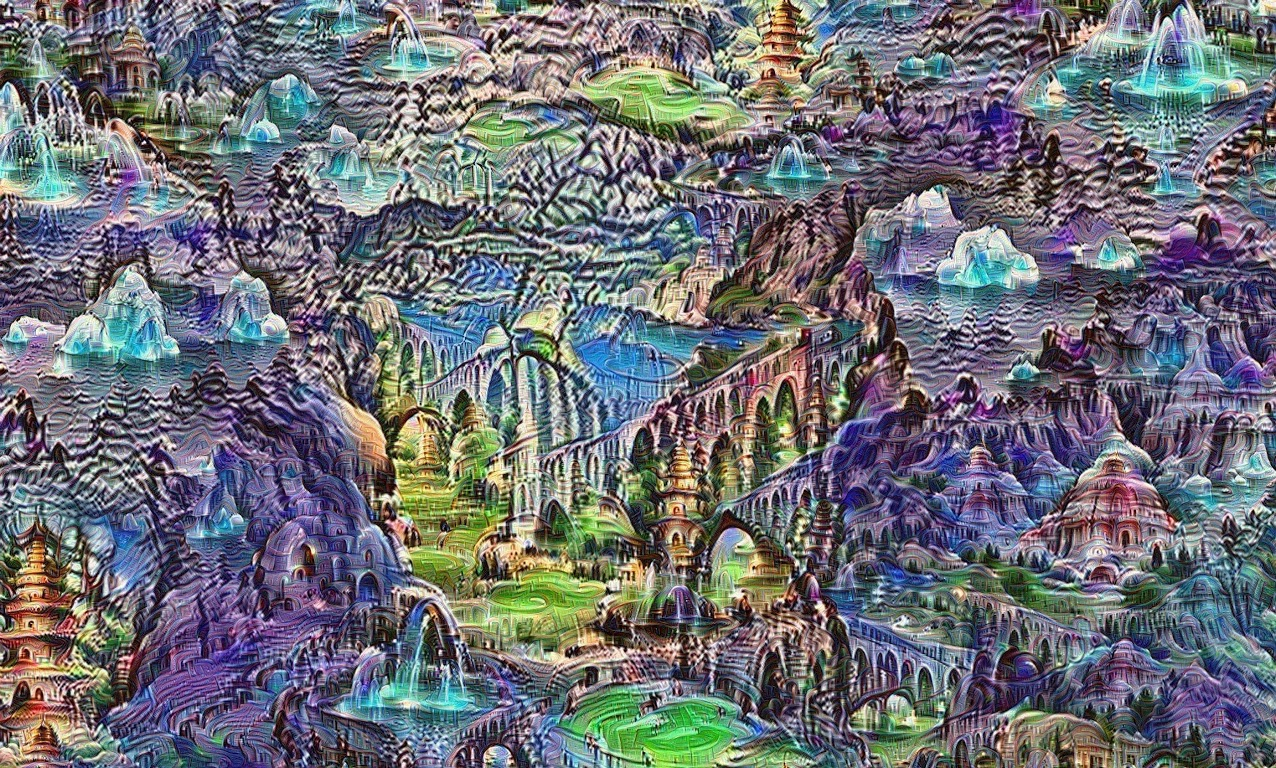
\includegraphics[width=\textwidth]{img/iterative_places}
\captionsetup{singlelinecheck=off,justification=raggedright}
\caption{Google Deep Dream \cite{Mordvintsev2015Inceptionism:Networks}}
\end{figure}
\end{frame}

% \begin{frame}{Measuring Evolvability}
% \begin{itemize}
%   \item amount of information able to acquire (different speeds of varying fitness function)\cite{Reisinger2005TowardsEvolvability} 
%   \item RMS distance in behavioral characterization space (population diversity), ``We approximate an individual’s capacity to generate
% future phenotypic variation by measuring phenotypic
% variability among a sample of the individual’s simulated off-
% spring (which are discarded). Such variability is quantified as
% the number of unique behaviors; in particular, each offspring
% is considered sequentially and added to a list of unique behaviors
% only if its behavior is significantly different from the
% behaviors of organisms already in the list. Two behaviors are
% considered different if the distance between them according
% to a domain-specific behavioral distance metric is above a
% pre-specified threshold'' \cite{Mengistu2016EvolvabilityIt}
%   \item ``a measurement of evolvability should characterize the
% amount of variability that can be accessed in an individual or population's genetic neighborhood; number of distinct phenotypes in a genetic neighborhood around individual; amounts to Monte Carlo sampling of the phenotypic space surrounding an individual \cite{Wilder2015ReconcilingEvolvability}
%   %\item \cite{Tarapore2015EvolvabilityBenchmarks}
% \end{itemize}
% \end{frame}



\end{document}
